% Document class report-template accepts either: project-plan or final-report option
\documentclass[final-report]{report-template}

% Packages I want to use in my report.
\usepackage{graphicx}
\usepackage{subfigure}
\usepackage{amsmath}
\usepackage{blindtext}
\usepackage{listings}
\usepackage{lmodern}
\usepackage{multirow}
\usepackage{appendix}
\usepackage{algorithm}
\usepackage{algpseudocode}
\usepackage[section]{placeins}
\usepackage{float}

% \def\LOGO{%
% \begin{picture}(0,0)\unitlength=1cm
% \put (3,-1) {\includegraphics[width=5em]{school_badge.png}}
% \end{picture}
% }

% Define and Set the code part style
\lstdefinestyle{mystyle}{
    backgroundcolor=\color{backcolour},   
    commentstyle=\color{blue!20!black!50!green},
    keywordstyle=\color{blue!70},
    numberstyle=\tiny\color{codegray},
    stringstyle=\color{codepurple},
    basicstyle=\footnotesize,
    breakatwhitespace=false,         
    breaklines=true,                 
    captionpos=b,                    
    keepspaces=true,                 
    numbers=left,                    
    numbersep=5pt,                  
    showspaces=false,                
    showstringspaces=false,
    showtabs=false,                  
    tabsize=2
}
\lstset{style=mystyle, escapeinside=``}


% Directory where I save my figures.
\graphicspath{{./figures/}}

% \university{Imperial College London}
% \department{Department of Earth Science and Engineering}
% \course{MSc in Applied Computational Science and Engineering}
% \title{Forecasting induced seismicity in Oklahoma}
% \author{Zhiyong Liu}
% \email{zl1220@ic.ac.uk}
% \githubusername{acse-liuzyon}
% \supervisors{Dr. Stephen P. Hicks}
\repository{https://github.com/acse-2020/acse2020-acse9-finalreport-liuzyon}


\begin{document}

\begin{titlepage}

\newcommand{\HRule}{\rule{\linewidth}{0.5mm}} % Defines a new command for the horizontal lines, change thickness here

\center % Center everything on the page

%----------------------------------------------------------------------------------------
%	HEADING SECTIONS
%----------------------------------------------------------------------------------------

\textsc{\LARGE Imperial College London}\\[1.5cm] % Name of your university/college
\textsc{\Large Department of Earth Science and Engineering}\\[0.5cm] % Major heading such as course name
\textsc{\large MSc in Applied Computational Science and Engineering}\\[0.5cm] % Minor heading such as course title

%----------------------------------------------------------------------------------------
%	TITLE SECTION
%----------------------------------------------------------------------------------------

\HRule \\[0.4cm]
{ \huge \bfseries Forecasting Induced Seismicity in Oklahoma}\\[0.4cm] % Title of your document
\HRule \\[1.5cm]
%----------------------------------------------------------------------------------------
%	AUTHOR SECTION
%----------------------------------------------------------------------------------------

\begin{minipage}{0.4\textwidth}
    \begin{flushleft} \large
    \emph{Author:}\\
    Zhiyong \textsc{Liu}\\ % Your name
    zl1220@ic.ac.uk\\
    GitHub: acse-liuzyon
    \end{flushleft}
    \end{minipage}
    ~
    \begin{minipage}{0.4\textwidth}
    \begin{flushright} \large
    \emph{Supervisor:} \\
    Dr. Stephen P. \textsc{Hicks}\\ % Supervisor's Name
    s.hicks@imperial.ac.uk
    \end{flushright}
\end{minipage}\\[2cm]

%----------------------------------------------------------------------------------------
%	LOGO SECTION
%----------------------------------------------------------------------------------------


\includegraphics[width=0.4\textwidth]{school.png}\\[3cm] % Include a department/university logo - this will require the graphicx package
 
%----------------------------------------------------------------------------------------


%----------------------------------------------------------------------------------------
%	DATE SECTION
%----------------------------------------------------------------------------------------

{\large \today}\\[1cm] % Date, change the \today to a set date if you want to be precise

\githubrepo  % GitHub repository
\vfill % Fill the rest of the page with whitespace

\end{titlepage}


% Metadata used for the title page.

\tableofcontents
\newpage

% Abstract
\section*{Abstract}
\addcontentsline{toc}{section}{Abstract}
Human activities can cause minor earthquakes, which are called induced earthquakes and most have a low magnitude. 
% Multi-year research by the United States Geological Survey (USGS) published in 2015 showed that most of large earthquakes occurred in Oklahoma may have been caused by injection of wastewater by industries.
In this project, a unique and rich dataset of industrial activities from regions combined with geological formation in Oklahoma are used and correlations between these factors and seismicity are confirmed.
With existing high-quality earthquake catalogues in these regions, statistically significant factors were selected by stepwise regression approach for models input.
A logistic regression model and a neural network model are generated to retrospectively forecast the seismicity. The performances about them are compared in various measures which denote neural network model has a better predicted ability and can be used in practice.
The depth to basement is founded mostly contributed to the seismicity.


\textbf{Key Words:} induced earthquakes, forecasting model, main factors for seismicity, machine learning methods.
\newpage

% Introduction section
\section{Introduction}
It is well known that humans can cause earthquakes through fluid injection and extraction. \citep{ellsworth2013injection} stated the understanding of the causes and mechanics of human-induced earthquakes. It includes wastewater injection, emerging oil and gas recovery technologies, and other indirect induced activities.
Such cases of induced seismicity have been recorded and proven in Oklahoma, where seismicity has been increased dramatically since 2010.
In cases like Oklahoma, because the rate of earthquakes was very low before high-rate wastewater injection, it is relatively easy to determine the fundamental causes of induced seismicity.
However, in tectonically-active areas, it is more challenging to distinguish between natural and triggered seismicity.
In tectonically active regions in the US, such as California, although oil and gas extraction has taken place for many decades, only a handful of studies have been published with a focus on these areas \citep{Hough2017WasTM}. 
Large-scale big-data and statistical approaches is one method to predict the locations where human triggered seismicity may be expected \citep{hincks2018oklahoma}.

To move onto an area with complex tectonic factors like California, we will use a less complicated testing environment to develop our big-data statistical approaches, like Oklahoma.
In this project, several unique and rich datasets of candidate factors from regions in Oklahoma are used to statistically evaluate and retrospectively forecast possible signatures of human-induced seismicity from existing high-quality earthquake in these regions. 
These datasets contain geological formation, injections, hydraulic fracturing activities and wells, each of which have millions of items.
In previous studies about induced earthquakes in Oklahoma, for instance, \citep{norbeck2018hydromechanical} associated the past injection trends with the seismicity patterns based on fluid flow and seismic physics to generate physical prediction models.
This project originally designed and implemented a feedforward neural network (FNN or NN) for induced seismicity forecasting, which effectively improves the performance of model fitting and prediction compared with logistic regression model (LR) also common-used in previous studies.
The superiority of our NN model was proven and their results about major factors to seismicity by two models were compared.

The detail introduction of geological visualization, feature selection and NN model will be delivered in Section~\ref{sec:software_description}. Section~\ref{sec:code_metadata} will describe metadata of code, including data files, code repository and dependencies.
Implementation about this project will be demonstrated in Section~\ref{sec:Implementation}. The results of models (LR and NN) and comparison as well as feature attribution will be stated in Section~\ref{sec:results}.
Finally, a conclusion of the project and future works will be presented in Section~\ref{sec:conclusion}. 




% Another section
\section{Software Description}
\label{sec:software_description}
% \subsection{Visualization: Matplotlib \& GeoPandas}
% GeoPandas \citep{jordahl2014geopandas} can make it easier researcher to process geospatial data in Python. It extends the datatypes in Pandas, which allows users to do spatial operations on geometric data.
% Matplotlib \citep{Hunter:2007} is a comprehensive library,  its main functions contain creating static, animated, and interactive visualizations for data in Python.
% Combining these two libraries, after setting the appropriate coordinate system, the data items can be mapped in spatial clearly by short code.

\subsection{Feature Selection: Stepwise Regression}
\label{sec:stepwise}
Stepwise Regression method is widely used to find which factors are important and which are not.
P-value is often used in stepwise regression to see if the patterns they measured were statistically significant. If the p-value of a statistical test is small enough, we are able to reject the null hypothesis of the test and the pattern measured is statistically significant.
The most common threshold for p is 0.05 \citep{ioannidis2018proposal}. For the variable whose p-value is greater than 0.05, we can assume that it is not statistically significant as shown in Appendix Fig~\ref{fig:p-value}.

In the construction of regression model, there usually exists a problem of high multicollinearity.
A little multicollinearity is not necessarily a serious problem that can be tolerated, but severe multicollinearity is a problem. Because it increases the variance of the regression coefficients which makes them unstable and difficult to interpret themselves.
A VIF between 5 and 10 means problematic and if the VIF is larger than 10, it is likely to poorly estimated the regression coefficients.

Considering both p-value and VIF, we used a forward stepwise logistic regression combined with VIF checking algorithm introduced in Algorithm~\ref{alg:cap}.

\begin{algorithm}
    \caption{Stepwise logistic regression with VIF checking}\label{alg:cap}
    \begin{algorithmic}
    \Procedure{SLR}{$candidate\_features$}
    \State $P\_THRESHOLD \gets 0.05$
    \State $VIF\_THRESHOLD \gets 5$
    \State $X \gets candidate\_features$
    \State $result \gets$ [ ]
    \For{\texttt{$feature$ in $X$}}
    \State $result.append(feature)$
    \State generate model with $result$
    \While{there exist some feature $N$ which $N.p\_value$ is greater than $P\_THRESHOLD$}
    \State eliminate feature with max $p\_value$ in $result$
    \State generate model with $result$
    \EndWhile

    \While{there exist some feature $N$ which $N.VIF$ is greater than $VIF\_THRESHOLD$}
    \State eliminate feature with max $VIF$ in $result$
    \State generate model with $result$
    \EndWhile
    \EndFor
    \EndProcedure
    \end{algorithmic}
    \end{algorithm}

% All features are initially excluded and a feature is added in each step whilst keeping current features satisfy p-value \textless 0.05. 
% This process continues until all features kept are statistically significant. Meanwhile, in each step, we also remain the VIF \textless 5 for current kept features even some new added feature is required to be eliminated. 

\subsection{Neural Network Construction: PyTorch} 
% Because logistic regression is so simple that it is difficult to model for nonlinear data or data with polynomial correlation, it is hard to deal with the complicated problem. 
% However, Neural network model has the ability to capture information in big-data and build incredibly complex models. 
% With the abilities of self-learning and high-speed for optimal solution, it easily achieves a higher performance compared with regression method.

PyTorch \citep{PyTorch} is a machine learning library for neural network in Python. 
It is open-source used for applications in natural language processing (NLP) and computer vision.
To define a neural network in PyTorch, it is pretty convenient to create a class that inherits from \textit{nn.Modules} within several rows of code. 
In the created class, user can define the layers of the network in the \textit{\_\_init\_\_} function and indicates how data will pass through the network in the \textit{forward} function. 

% Facebook's AI Research lab (FAIR) \citep{patel2018two} mostly developed it and recommended it with two features:
% \begin{itemize}
%     \item Accelerated computing for Tensors (like Numpy) via GPU.
%     \item Provide neural networks which are built on a system supportring automatic differentiation.
%   \end{itemize}
% Pytorch provides a class called Tensor (\textit{torch.Tensor}) to store and manipulate numerical homogeneous multidimensional rectangular arrays. 
% They are tailor-made for datasets in machine learning. Pytorch Tensors are similar to NumPy Arrays, but it supports to be manipulated on a CUDA-capable Nvidia GPU \citep{paszke2019pytorch} for acceleration.

% Figure~\ref{fig:neural_network_example} is the model created above trained on the playground online through TensorFlow. 

% \begin{lstlisting}[language=Python]    
%     # Define NN model
%     class NeuralNetwork(nn.Module):
%         def __init__(self):
%             super(NeuralNetwork, self).__init__()
%             self.flatten = nn.Flatten()
%             self.linear_relu_stack = nn.Sequential(
%                 nn.Linear(4, 8),
%                 nn.ReLU(),
%                 nn.Linear(8, 8),
%                 nn.ReLU(),
%                 nn.Linear(8, 2),
%                 nn.ReLU()
%             )
    
%         def forward(self, x):
%             x = self.flatten(x)
%             logits = self.linear_relu_stack(x)
%             return logits
    
%     model = NeuralNetwork().to(device)
% \end{lstlisting}

\subsection{Feature Attribution: Captum}
Feature attribution is the technique to investigate how much each feature in the model contributes to the prediction for given dataset fitting. 
Because models in machine learning are more complicated and lack of transparency, the interpretability approaches for these models have becoming increasingly important.
Captum is an interpretability and understanding library for models in PyTorch.
It provides a lot of advanced algorithms, including Integrated gradients \citep{sundararajan2017axiomatic},  DeepLIFT \citep{shrikumar2017learning}, Feature Ablation and Gradient SHAP \citep{lundberg2017unified} used in this project. 
These Captum provide users a convenient way to know about the contributions of features to a models' output through these algorithms.
% \subsubsection{Integrated Gradients}
% Integrated gradients \citep{sundararajan2017axiomatic} represent the integral of gradients with respect to inputs along the path from a given baseline to input. The integral can be approximated using a Riemann Sum or Gauss Legendre quadrature rule. Formally, it can be described as follows in Equation \eqref{equ:inreGrad}:

% \begin{equation}
%     IntegratedGrads_{i}(x) ::= (x_{i} - x_{i}^{'}) \times   \int_{\alpha=0}^1 \frac{\partial F(x^{'}+\alpha \times (x-x^{'}))}{\partial x_{i}} d\alpha  \label{equ:inreGrad}    
% \end{equation}

% Integrated Gradients along the i-th dimension of input X. Alpha is the scaling coefficient.
% The cornerstones of this approach are two fundamental axioms, namely sensitivity and implementation invariance.

% \subsubsection{Gradient SHAP}
% Gradient SHAP \citep{lundberg2017unified} is a gradient method to compute SHAP values, which are based Shapley values proposed in cooperative game theory. Gradient SHAP adds Gaussian noise to each input sample multiple times, selects a random point along the path between baseline and input, and computes the gradient of the outputs with respect to those selected random points. 
% The final SHAP values represent the expected value of gradients $\times$ (inputs - baselines).
% The computed attributions approximate SHAP values under the assumptions that the input features are independent and that the explanation model is linear between the inputs and given baselines.

% \subsubsection{DeepLIFT}
% DeepLIFT \citep{shrikumar2017learning} is a back-propagation based approach that attributes a change to inputs based on the differences between the inputs and corresponding references (or baselines) for non-linear activations.
% As such, DeepLIFT seeks to explain the difference in the output from reference in terms of the difference in inputs from reference.
% DeepLIFT uses the concept of multipliers to "blame" specific neurons for the difference in output. The definition of a multiplier is as follows:

% \begin{equation}
%     m \Delta x \Delta t = \frac{C \Delta x \Delta t}{\Delta x}  \label{equ:DeepLIFT}    
% \end{equation}
% x is the input neuron with a difference from reference $\Delta x$, and t is the target neuron with a difference from reference $\Delta t$. C is then the contribution of $\Delta x$ to $\Delta t$.

% \subsubsection{Feature Ablation}
% Feature ablation is a perturbation-based approach to compute attribution, involving replacing each input feature with a given baseline / reference value (e.g. 0), and computing the difference in output. 
% Input features can also be grouped and ablated together rather than individually. This can be used in a variety of applications. 
% For example, for images, one can group an entire segment or region and ablate it together, measuring the importance of the segment (feature group).

\subsection{Model Evaluation Measures}
\label{sec:model_evaluate_measures}
The measures we used for model evaluation will be introduced in this section. 
These measures contain accuracy, confusion matrix, precision, recall, F1 score, ROC curve and AUC value.

\subsubsection{Accuracy, Precision, Recall and F1 Score}
\label{sec:APRF}
In confusion matrix, it has four cells which represents TN, FN, FP, TP.
The meanings of these four types are listed below:
\begin{itemize}
    \item TN: Prediction is 0 and true is 0. 
    \item FN: Prediction 0 but true is 1. 
    \item FP: Prediction is 1 but true is 0.
    \item TP: Prediction is 1 and true is 1.
\end{itemize}

The accuracy, precision, recall, F1 score are calculated based on the four types in confusion matrix.
According to the confusion matrix, they can be calculating by Equation \eqref{equ:accuracy}\eqref{equ:precision}\eqref{equ:recall}\eqref{equ:F1}.

\begin{equation}
    Accuracy ::= \frac{TN + TP}{TN+FN+FP+TP}  \label{equ:accuracy}    
\end{equation}

\begin{equation}
    Precision ::= \frac{TP}{TP+FP}  \label{equ:precision}    
\end{equation}

\begin{equation}
    Recall ::= \frac{TP}{TP+FN}  \label{equ:recall}    
\end{equation}

\begin{equation}
    F1 ::= 2 \times \frac{Precision \times Recall}{Precision+Recall}  \label{equ:F1}    
\end{equation}

The accuracy is a common measure in model evaluation, and it is an intuitive representation of whether the model is capable of making accurate predictions.
However, it is easily affected by the imbalance of the samples. For example, there are a total of 100 samples and 90 of them are positive samples.
If the model predicts all samples to positive sample, the accuracy can reach up to 90\%, but such a model is meaningless obviously.  

Precision states from the perspective of prediction results, it describes how many of the positive predictions predicted by the binary classifier are accurate. 
Recall states from the perspective of real results, it describes how many real positive samples are recalled by the binary classifier.
Precision and Recall are contradictory with each other. Generally, recall tends to be low when precision is high.
For earthquake prediction, we focus more on seismic samples rather non seismic samples. 
Therefore, we have two expectations:
\begin{itemize}
    \item we want a high precision because it means more predictions in seismic predictions are correct.  
    \item we want a high recall because it means more actual seismic samples are selected out by the model.
    
    Note: Seismic prediction here refers to the prediction whose result is a seismic area.
\end{itemize}

In order to take these two expectations into consideration, we introduced F1 score, which is the harmonic mean \citep{chhikara1988inverse} of precision and recall.
If the F1 score is high, it means model highly meet both expectations.

\subsubsection{ROC Curve and AUC Value}

\begin{equation}
    FPR ::= \frac{FP}{N} = \frac{FP}{FP+TN}  \label{equ:FPR}    
\end{equation}

\begin{equation}
    TPR ::= \frac{TP}{P} = \frac{TP}{TP+FN}  \label{equ:TPR}    
\end{equation}

We also used the Receiver Operating Characteristic Curve (ROC) to evaluate LR model and NN model. 
The ROC curve is drawn by a series of different dichotomies (dividing values or determining thresholds). 
The abscissa represents the false positive rate FPR (1-specificity) shown in Equation \eqref{equ:FPR} and the ordinate represents the true positive rate TPR (sensitivity) shown in Equation \eqref{equ:TPR}. 

ROC has the superiority of independence of class distribution, which is suitable for evaluation with unbalanced datasets.
We can see why it has this advantage from their equations. 
TRP used TP and FN, which both belongs to second row in confusion matrix. It only concentrates on positive samples (P, which was represented by the second row in confusion matrix). 
FRP used FP and TN, which both belongs to first row in confusion matrix. It only concentrates on negative samples (N, which was represented by the first row in confusion matrix). Therefore, even if the number of P or N changes, they do not affect each other.
That is to say, even if the ratio of positive to negative samples changes greatly, the ROC curve does not change greatly. However, this is not a feature of the previous measures in Table~\ref{tab:Indicators_by_confusion_matrix}. 
The performance of the classification model can also be represented intuitively by the area under the ROC curve (AUC). AUC ranges in value from 0 to 1. A model has an AUC of 0.0 if its predictions are 100\% wrong; In reverse, if it is 100\% accurate, it has an AUC of 1.0.

\section{Code Metadata}
\label{sec:code_metadata}
This project was built under macOS Catalina environment with Jupyter Notebook 6.0.3 and Python 3.7.6.
The information of libraries and their usages are listed in Table~\ref{tab:library_dependency}.

In the GitHub repository, source code files (\textit{.ipynb}) are stored in the \textit{src} directory, including two main parts, which are feature extraction and prediction model. An additional file \textit{visualization.ipynb} is used for some figures in this report.
The dataset files (\textit{.csv}) generated from feature extraction part are located at \textit{data} directory. The models (\textit{.pt}) generated from prediction part are located at the \textit{model} directory.

\section{Implementation}
\label{sec:Implementation}


\subsection{Data Processing and Spatial visualization}
\label{sec:dpsv}
In the initial phase of project, we imported all the available datasets (earthquake data, geological data, hydraulic fracturing data, injection data, well data).
The metadata of earthquake dataset was exported from \textit{Oklahoma Geological Survey Earthquake Catalog Download Tool} \citep{walter2020oklahoma}.
The metadata of injection dataset was exported from \textit{Oklahoma Corporation Commission} \citep{OklahomaCorporationCommission}.
The metadata of hydraulic fracturing dataset was exported from \textit{FracFocus} \citep{FracFocusChemicalDisclosureRegistry}.

We then preprocessed the imported datasets, which includes missing values processing and data selecting by date.
The date of injection dataset we imported was in the range of 2011 to 2020. Because the data files \textgreater 2019 supported by the \textit{Oklahoma Corporation Commission} are still under review and corrections are being made as warranted, those files are currently incomplete and subject to change. Therefore, we only used the data between 2011 and 2018.
Due to date limitation of injection data, we set the interest time in the period of 2011 to 2018 for all datasets.
We set the interest area to the area whose longitude ranges in (-99.5W, -96W) and latitude ranges in (35.0N, 37.0N) shown as red box in Figure~\ref{fig:earthquake_plot}, which is an available spatial scope provided by all datasets.
We visualized all the data by \textit{matplotlib} and \textit{geopandas} module in the interest area and date. The geodetic coordinate system we used for mapping in this project is 'EPSG:4326' \citep{epsg}, which is the most popular coordinate system. 
The geological formation (depth to basement) along with various activities (seismicity, injections, wells, hydraulic fracturing) are shown in Fig~\ref{fig:activity}.

% The core of visualization code for all dataset is similar and earthquake visualization is shown in the below code part:
% \begin{lstlisting}[language=Python]
%     earthquake_geometry = [Point(xy) for xy in zip(earthquake_df['longitude'], earthquake_df['latitude'])]
    
%     earthquake_geo_df = gpd.GeoDataFrame(earthquake_df, crs = "EPSG:4326", geometry = earthquake_geometry)

%     fig, ax = plt.subplots(figsize=(20, 20), dpi=300)
%     oklahoma_map.plot(ax=ax, alpha=0.4,color='grey')
%     earthquake_geo_df.plot(column='magnitude',ax=ax, alpha=0.5, legend=True, markersize=10)

%     plt.title('Earthquake (magnitude>=2) in Oklahoma', fontsize=15,fontweight='bold')
%     plt.xlim(-99.5, -96.0)
%     plt.ylim(35.0, 37.0)
%     plt.show()
% \end{lstlisting}

\subsection{Spatial Griding and Features Extraction}
For the interest area (longitude ranges in (-99.5W, -96W) and latitude ranges in (35.0N, 37.0N)), we divided it into $40 \times 40$ grids. 
The size (40 $\times$ 40) of griding depended on the adequacy of generated dataset and the suitable size of the unit region.
In this case, it generated 1600 data items for model construction and each of them has the distance of 8km in x-direction and 6 km in y-direction.

Then, we counted the values of all features and target for each grid by the various data from Section~\ref{sec:dpsv} to generate the dataset.
This dataset files were generated in \textit{.csv} and saved in \textit{data} directory.
The features and target of this dataset is shown in Table~\ref{tab:feature_generated}.
% \begin{itemize}
%     \item \textit{injection\_number [entry]}: The number of injections in this grid.
%     \item \textit{injection\_vol\_sum [BPD]}: The sum of injection volume in this grid.
%     \item \textit{injection\_psi\_sum [PSI]}: The sum of injection pressure in this grid.
%     \item \textit{injection\_depth\_avg [m]}: The mean of injection depth in this grid.
%     \item \textit{injection\_above\_basement\_number [entry]}: The number of injections whose depth are shallow than the basement in this gird.
%     \item \textit{injection\_under\_basement\_number [entry]}: The number of injections whose depth are deeper than the basement in this gird.
%     \item \textit{injection\_close\_to\_basement\_500\_number [entry]}: The number of injections whose depth is within 500 metres of basement.
%     \item \textit{injection\_close\_to\_basement\_1000\_number [entry]}: The number of injections whose depth is within 1000 metres of basement.
%     \item \textit{active\_well\_number [entry]}: The number of working wells in this grid.
%     \item \textit{well\_depth\_avg [m]}: The mean of well depth in this grid.
%     \item \textit{well\_above\_basement\_number [entry]}: The number of working wells whose depth are shallow than the basement in this grid.
%     \item \textit{well\_under\_basement\_number [entry]}: The number of working wells whose depth are deeper than the basement in this grid.
%     \item \textit{well\_close\_to\_basement\_500\_number [entry]}: The number of wells whose depth is within 500 metres of basement.
%     \item \textit{well\_close\_to\_basement\_1000\_number [entry]}: The number of wells whose depth is within 1000 metres of basement.
%     \item \textit{depth\_to\_basement\_avg [m]}: The mean of the depth to the basement in this grid.
%     \item \textit{hf\_number [entry]}: The number of hydraulic fracturing activities in this grid.
%     \item \textit{hf\_base\_water\_volume\_sum [BPD]}: The sum of volume by hydraulic fracturing with water
%     \item \textit{hf\_base\_nowater\_volume\_sum [BPD]}: The sum of volume by hydraulic fracturing with nowater
%     \item \textit{earthquake\_occurrence [0 or 1]}: If earthquake occurred in this grid. 0: not occured; 1: occurred.
% \end{itemize}



\begin{figure}
    \begin{center}
        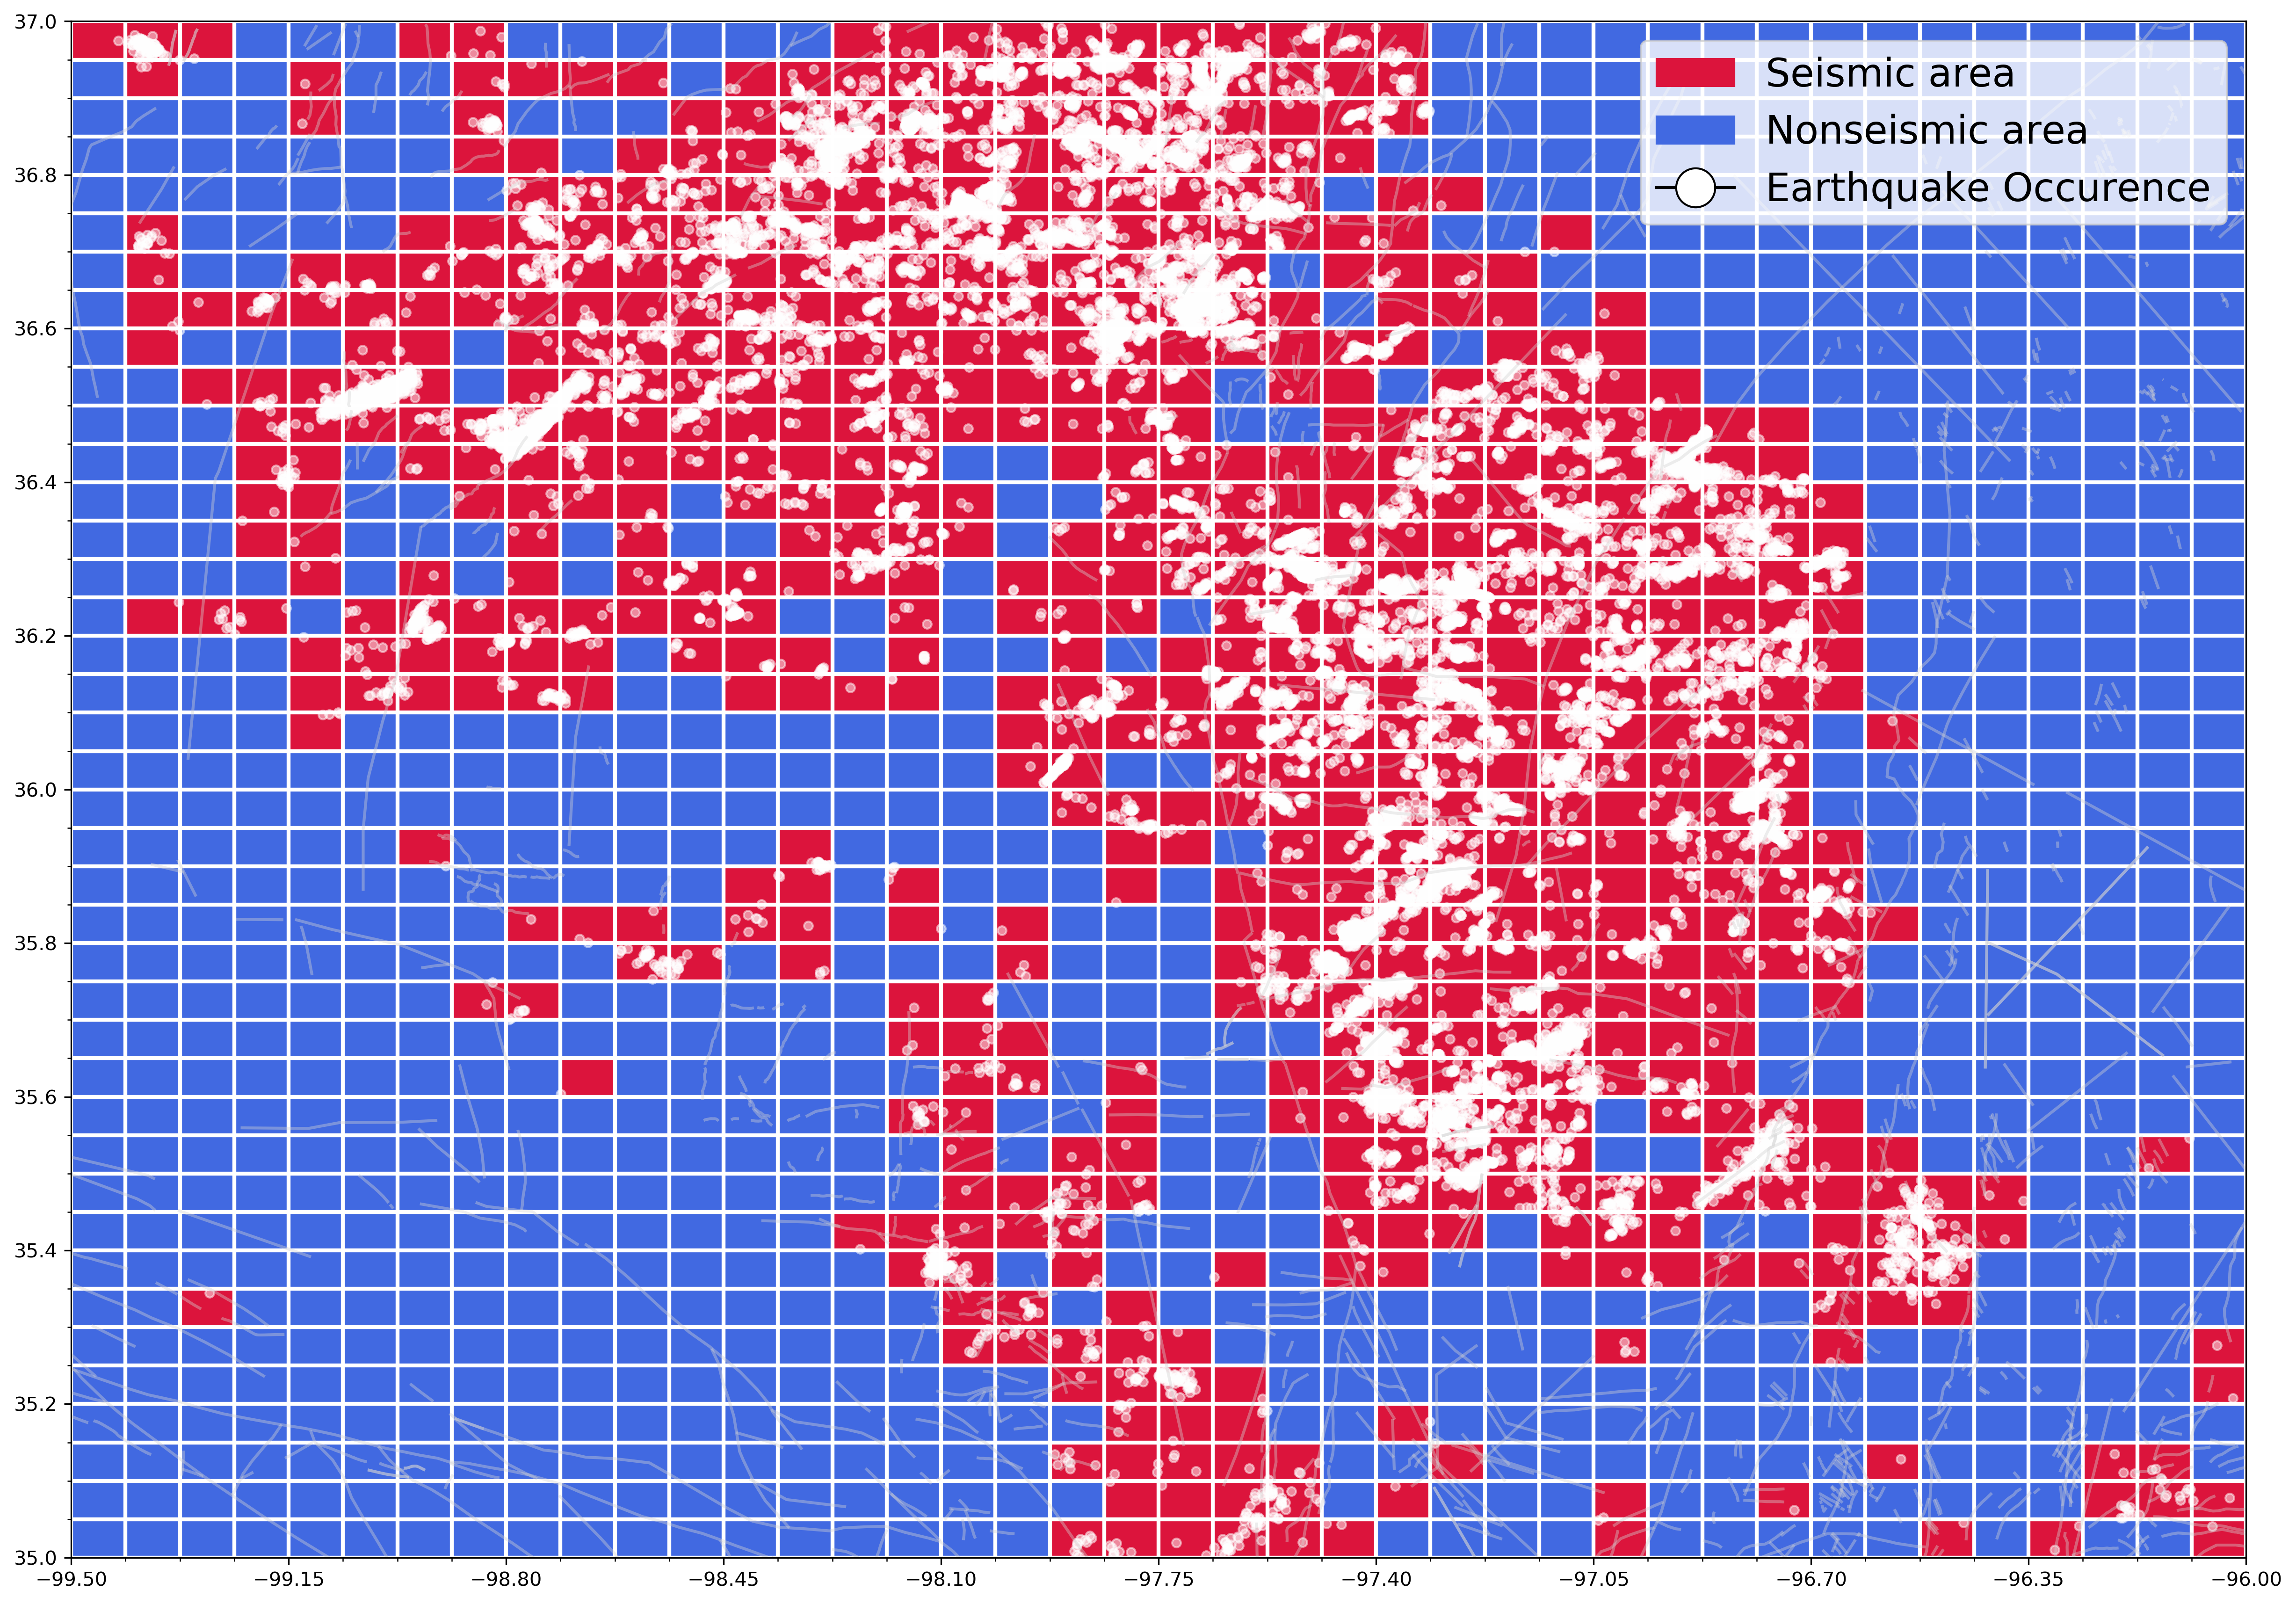
\includegraphics[width=1\textwidth]{target_mapping.png}
    \end{center}
    \caption{\label{fig:target_mapping} Target variable of earthquake occurrence within the interest area in Oklahoma (The white lines display the gridding regions, with a spacing in the x direction of 8 km and the y direction of 5.5 km. The white points denote the earthquake occurrences.
    The red region denotes it has seismicity in this region and blue region denotes it does not have seismicity in this region).}
\end{figure}
After this statistical process, we obtained a dataset in terms of spatial distribution. Each of item represents a subarea of our interest area and contains the values of various candidate features.
The target variable is set by seismicity, which represents the seismicity in spatial distribution. We made each grid region a value of 1 if there was at least one (magnitude\textgreater2) earthquake occurred during 2011 to 2018. 
Otherwise, if no earthquake occurred in this grid region, we assigned it a value of 0. The griding result of the earthquake occurrence (target) from 2011 to 2018 is shown in Figure~\ref{fig:target_mapping}. 
The class distribution with whole dataset is shown in Figure~\ref{fig:class_label}. There are 920 nonseismic grid regions with label '0' and 680 seismic grid regions with label '1'.

\begin{figure}
    \begin{center}
        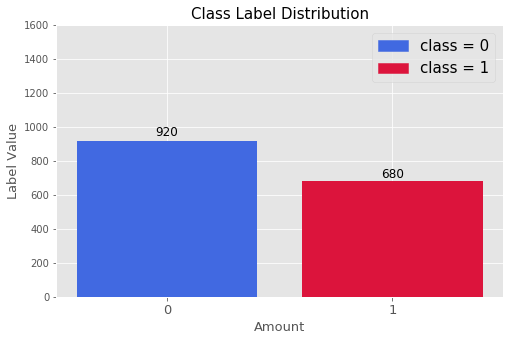
\includegraphics[width=0.7\textwidth]{class_label.png}
    \end{center}
    \caption{\label{fig:class_label} Class label distribution in whole dataset (0: nonseismic region; 1: seismic region).}
\end{figure}

\subsection{Stepwise Feature Selection Approach}
\label{sec:SFSA}
As some activities were strongly overlapped in spatial distribution, they might have a high degree of multicollinearity. 
We calculated the feature similarity on all features based on Pearson \citep{benesty2009pearson} correlation coefficients and generated a heatmap as Appendix Figure~\ref{fig:heatmap}.
In general, we consider a high degree of collinearity between two features with a coefficient greater than 0.9, like 'active\_well\_number' and 'well\_under\_basement\_number'.
To select statistically significant features and deal with high multicollinearity problem, we used the forward stepwise approach with VIF checking algorithm introduced in Section~\ref{sec:stepwise}. 
After this process, we eliminated statistically insignificant features and also solved the problem of high multicollinearity between features. 
% The result of features selecting is shown in Figure~\ref{fig:stepwise}. 

\subsection{Logistic Regression Model}
\label{sec:LRM}
With the selected features in Section~\ref{sec:SFSA}, we constructed a multiple logistic regression model in this part, which used the features selected as independent variables and earthquake occurrence as the target variable.
We standardized and normalized all input features by z-score normalization \citep{patro2015normalization} to reduce data skewness and bring all features on the same scale. 
The normalization makes it feasible to interpret the relative differences of LR model coefficients.

We split the dataset into train dataset and test dataset with the ratio of 4:1, which respectively have 1280 and 320 samples (Each sample is associated with one gridding region in the interest area). In the build process of LR model, we used \textit{sklearn.linear\_model.LogisticRegression} to construct and fitted our LR model with training data by \textit{fit} function.
%  which achieved the accuracy of 72.5\% on the test dataset.
% The core part of code is shown in below:
% \begin{lstlisting}[language=Python]
%     X_train,X_test,y_train,y_test = train_test_split(X,Y,train_size=0.9, random_state=42)
%     model = LogisticRegression()
%     model.fit(X_train,y_train)
%     model.score(X_test,y_test)
% \end{lstlisting}
% After fitting the model and testing, we checked the coefficients for all input features by \textit{model.coef\_[0]} and plot them in Figure~\ref{fig:feature_attribution}. With the trained logistic regression model, we used the whole dataset to predict and compared output labels with true labels, which is shown as sub-figure(b) in Figure~\ref{fig:mapping_comparison}.

\subsection{Neural Network Model}
\label{sec:NNM}
\subsubsection{Architecture}
In this project, we used a neural network model which has its input layer with 7 neurons, two hidden layers of 8 neurons per layer and an output layer with 2 neurons as shown in Figure~\ref{fig:neural_network_model}. 
In general, 1 to 5 hidden layers and same number of neurons for all hidden layers will be enough for most problems.
Therefore, we chose to use two hidden layers and each layer has 8 neurons since we did not have too many input features.
The input features used were also based on the feature selecting result in Section~\ref{sec:stepwise}, so we had seven input features for our training model and it was taken for granted that we set the number of input neurons to 7, which represented each input feature.
Because the earthquake prediction problem is a binary classification, we used 2 neurons in output layer. Each output neuron represents one class. The output represents the probability of the classes (earthquake or no earthquake). 
In the end, the SoftMax activation function \citep{dunne1997pairing} are performed on the output layer, which make the final probabilities of classes sum to 1 (SoftMax we implemented in training function rather than in definition of NN class).

We used PyTorch to conveniently define the neural network model corresponding to architecture in Figure~\ref{fig:neural_network_model} by the code in Appendix Section~\ref{sec:NN_code}.
It implemented three linear transformations, which represented input layer $\rightarrow$ $1^{st}$ hidden layer, $1^{st}$ hidden layer $\rightarrow$ $2^{nd}$ hidden layer and $2^{nd}$ hidden layer $\rightarrow$ output layer.
Each transformation performs a linear transformation to input data in the form of $y = xA^{T} + b$. \textit{x} represents the vector of neuron values before transformation and \textit{y} represents a vector of neuron values after transformation.
\textit{A} represents the weights multiplied in linear transformation (like coefficients in regression) and \textit{b} represents the vector of bias. 
Our input layer corresponding to input features, so we set the \textit{n\_input} variable in code to 7. 
Our output layer corresponding to output target class, so we set the \textit{n\_output} variable in code to 2.
The \textit{\_\_init\_\_} function defines the architecture of neural network. The \textit{forward} function in the code represents the process of propagation.


\subsubsection{Configuration}
Because this prediction problem is binary classification problem, we used the cross-entropy \citep{de2005tutorial} as the loss function of model.
By lots of training attempts, we finally used a set of hyperparameters which make the model performance in a best level.

Generally, the best performance was reached by mini-batch sizes in the range of 2 to 32. In training attempts, we found that the model performed best when the batch size was set to 8.
For the epoch size, we started from 400 epochs which is a large selection for epoch size and stopped early to halt training when performance stopped improving.
The selection of the learning rate is also significant, we started with a pretty low value ($10^{-6}$) and slowly multiply it by 10 until it reaches 1 to determine which rate served well for our earthquake prediction problem. 
We found $10^{-3}$ is best and retrained our model using this optimal learning rate.
For the optimizer used in our model, we decided to use Adam optimizer, which tends to excuse bad learning late and other non-optimal hyperparameters compared with most common used SGD optimizer.

The configuration which is called hyperparameters in machine learning is summarized below:

\begin{itemize}
    \item \textit{learning rate}: $10^{-3}$
    \item \textit{batch size}: 8
    \item \textit{epoch}: 200
    \item \textit{optimizer}: Adam
    \item \textit{loss function}: cross entropy
\end{itemize}

\begin{figure}
    \begin{center}
        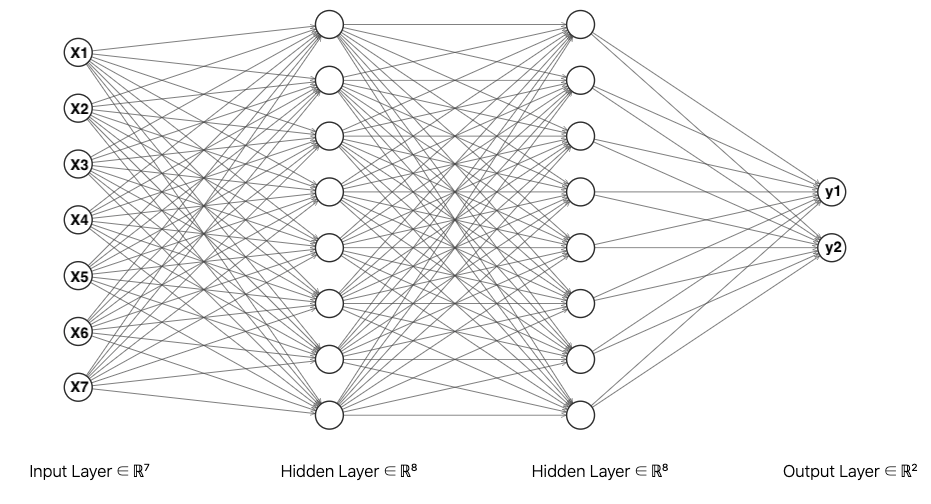
\includegraphics[width=1\textwidth]{neural_network_model.png}
    \end{center}
    \caption{\label{fig:neural_network_model} Constructed feedforward neural network model architecture.}
\end{figure}

\subsubsection{Training}
\label{sec:NN_training}
We initially divided the dataset into training dataset and testing dataset and normalized them as we done before fitting logistic regression model in \ref{sec:LRM}.
We trained the NN model with the optimized hyperparameters above.
For each epoch, we trained using the whole training dataset and tested the accuracy of current model in testing dataset.  
We used \textit{torch.utils.data.DataLoader} to load the training dataset and testing dataset.
Every time we loaded a batch (8 samples) of training data and input into model for propagation, the outputs were compared with the labels. 
According to loss of current batch, we updated the weights in model by \textit{optimizer.step()}.
After training by each epoch, we calculate the accuracy of NN model on training dataset and testing dataset respectively and updated the loss of them in log plot. 
The training process of our NN model is shown in Appendix Figure~\ref{fig:training_process}.


\section{Results and Discussion}
\label{sec:results}
This section will analyze the results from Section~\ref{sec:Implementation}.

\subsection{Visualization}
\label{sec:visualization_result}

\begin{figure}
    \begin{center}
        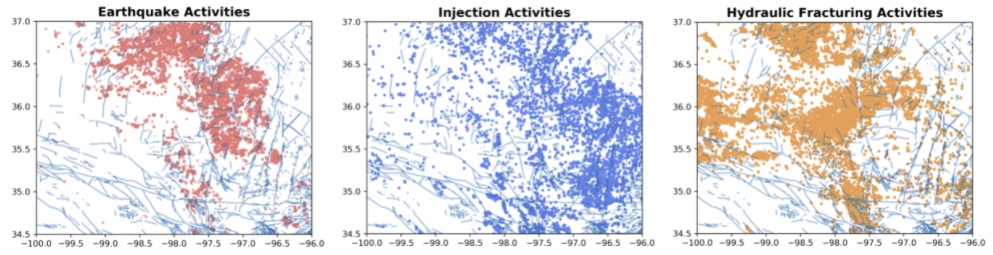
\includegraphics[width=1\textwidth]{activity.png}
    \end{center}
    \caption{\label{fig:activity} Activities during 2011 to 2018 in interest area from Oklahoma (The three black boxes in (a)(b) denote similar dense distribution between seismicity and injections).}
\end{figure}

Through these activities distribution in Fig~\ref{fig:activity}, we can find a rough spatial correlation between some of them.
We firstly compare the depth to basement with earthquake activities. In the Figure~\ref{fig:activity} (e) it shows lower left region has larger depth value and upper right region almost has 0 value,
which means the lower left region of interest area has a thicker softer sedimentary rocks than upper right region.
This corresponds to earthquake occurrences more in the upper right region than in the lower left region of interest area.
It can be inferred that the induced seismicity may be related to depth to basement. 
Besides, injection activities are similar to earthquakes activities in spatial distribution. 
As the Figure~\ref{fig:activity} shows, three black rectangular regions (marked by 1 to 3) represent the seismicity and injections dense area respectively, which are highly similar in spatial distribution, even in small area as rectangular area 3. 
By the high similarity, we can conclude that the induced seismicity has high correlation with injection activities.
However, in terms of the hydraulic fracturing activities and well spatial data, we cannot find some relation between induced earthquake and them and we need to explore and interpret through the model generated.

\subsection{Features Selection}
The process of features selection with stepwise regression approach is shown in Appendix Section~\ref{sec:feature_selection_process} and the result of feature selecting along with their p-value and VIF is shown in Figure~\ref{fig:stepwise}.

\begin{figure}[H]
    \begin{center}
        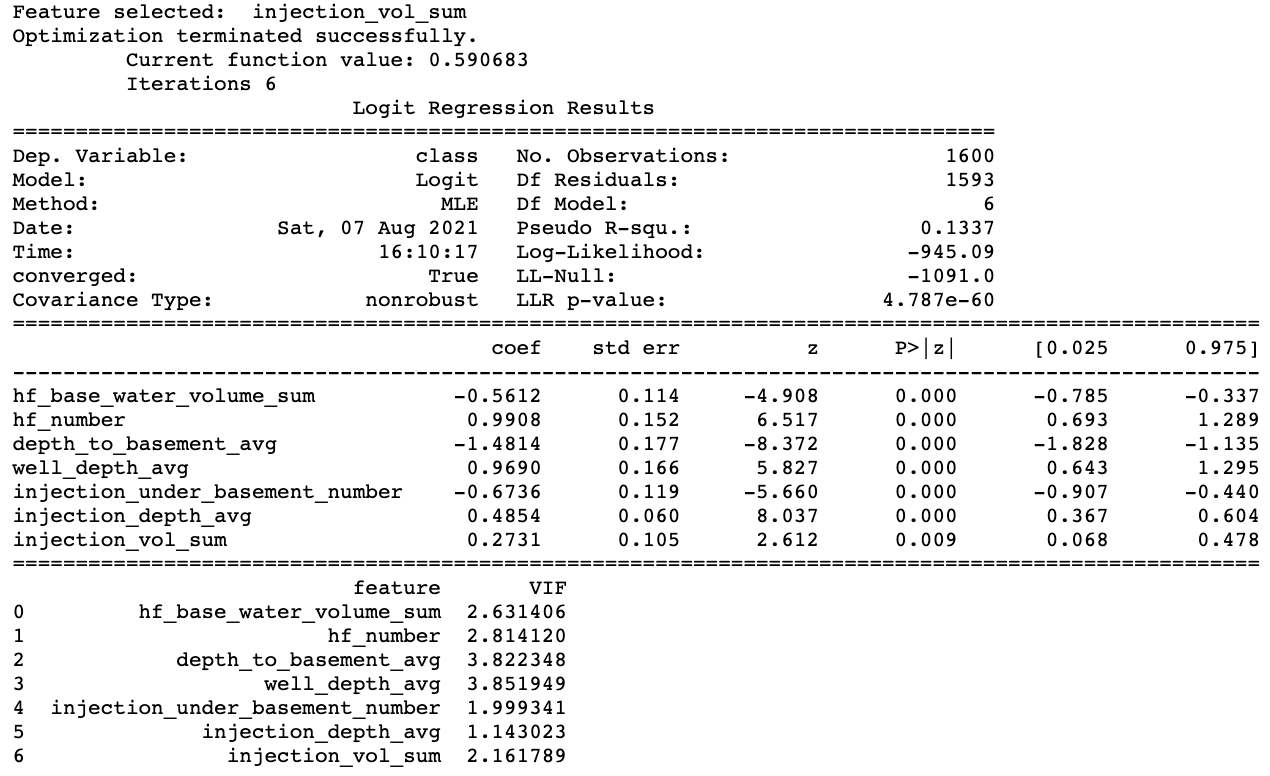
\includegraphics[width=0.9\textwidth]{stepwise.png}
    \end{center}
    \caption{\label{fig:stepwise} Result of feature selection using stepwise regression with VIF checking.}
\end{figure}

We can see all the selected features by stepwise regression approach meet the requirement of p-value \textless 0.05 and VIF \textless 5.
This means we successfully eliminated the features which are not statistically significant and there is no high multicollinearity in all features selected.  

\subsection{Model Evaluation and Comparison}
\label{sec:model_evaluate_comparison}
By the Section~\ref{sec:LRM} and Section~\ref{sec:NNM}, we fitted the LR model and trained the configured NN model on the training dataset. 
Their prediction accuracy on testing dataset achieved at 72.18\% and 80.3\% respectively. 
It denotes that NN model performs better than LR model in terms of unseen dataset and have better ability of generalization.
Besides, we finally used these models to test on the whole dataset, which contains all the grids point of interpret area. The results on whole dataset will be evaluated in this section.
The confusion matrixes of results by these two models are shown on Figure~\ref{fig:confusion_matrix}. The measures we introduced in Section~\ref{sec:model_evaluate_measures} to evaluate models are calculated based on confusion matrices and shown in Table~\ref{tab:Indicators_by_confusion_matrix}.
\begin{figure}
    \begin{center}
        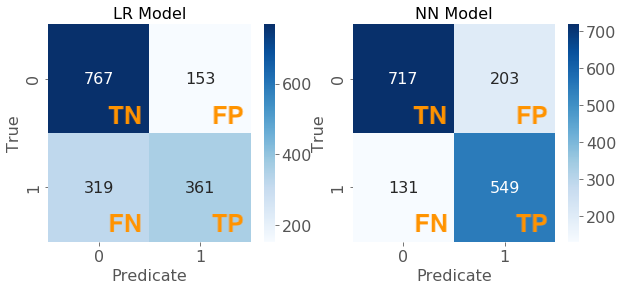
\includegraphics[width=0.8\textwidth]{confusion_matrix.png}
    \end{center}
    \caption{\label{fig:confusion_matrix} Confusion matrices of prediction results by LR model and NN model.}
\end{figure}

\begin{table}
    \centering
    \caption{Measures calculated using confusion matrices by LR model and NN model}
    \label{tab:Indicators_by_confusion_matrix}
    \begin{tabular}{|c|c|c|c|c|}
    \hline
    Model\textbackslash{}Indicator & Accuracy   & Precision & Recall & F1-score \\ \hline
    Logistic Regression Model      & 0.705 & 0.702     & 0.530  & 0.604    \\ \hline
    Neural Network Model           & 0.791  & 0.730     & 0.807  & 0.766    \\ \hline
    \end{tabular}
    \end{table}
    
The accuracy denotes the proportion of all correct predictions in the total predictions. 
We can see for all regions in interest area, the prediction accuracy of NN model (79.1\%) is 9 percent higher than LR model (70.5\%).
Through the accuracy comparison for LR model and NN model in Table~\ref{tab:Indicators_by_confusion_matrix}, it shows that for a task of predicting a class label of one region in interest area, NN model have a higher prediction accuracy. 
Unfortunately, the samples in our dataset are not balanced in the ratio of 2:3 as shown in Figure~\ref{fig:class_label}.
Therefore, using the accuracy to evaluate has great defects introduced in Section~\ref{sec:APRF} in this earthquake prediction problem, which may have high accuracy but meaningless.  

We also compare two models in precision and recall. 
According to the Table~\ref{tab:Indicators_by_confusion_matrix}, the precisions of two models are similar.
This denotes that for all seismic predictions, two models have the similar ability to predict correctly.
However, we found the recall of NN model is much higher than that of LR model, which is 0.53 (LR) and 0.807 (NN).
This means that for one real seismic region, the NN model has the probability of 80.7\% but LR model only have a probability of 53\% to predict correctly. The LR model shows a terrible performance for binary classification problem concentrating on real seismic regions.
Furthermore, in order to meet our two expectations mentioned simultaneously in Section~\ref{sec:APRF}, we also introduced the F1 score. As Table~\ref{tab:Indicators_by_confusion_matrix} shows, LR model has the F1-score of 0.604 and NN model has the F1-score of 0.766.
It shows that NN model indeed satisfied expectations that it can both make more accurate predictions and select out more actual seismic samples.

\begin{figure}
    \begin{center}
        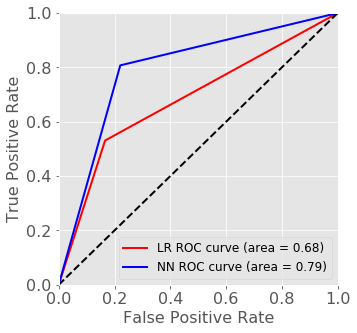
\includegraphics[width=0.5\textwidth]{ROC_curve.png}
    \end{center}
    \caption{\label{fig:ROC_curve} ROC curves by LR model and NN model (Black diagonal line represents random guessing in binary classification problem).}
\end{figure}

In ROC curve, the diagonal line (black line in Figure~\ref{fig:ROC_curve}) represents random guessing. 
Therefore, a model with ROC curve below diagonal has the performance inferior to random guessing.
When we evaluate model on ROC, we hope that the TP rate to be high when the FP rate is low because we want no false positive and no false negative. This state is just the ideal perfect state for a binary classification problem (FPR = 0, TPR = 1, which is (0, 1) in left top corner in Figure~\ref{fig:ROC_curve}), where all the predictions are correct.
In other words, the steeper the ROC curve or the closer to left top corner, the more accurate the model is.
From the Figure~\ref{fig:ROC_curve}, we can see both LR model curve and NN model curve are above the diagonal line, which means these two models are better than random guessing.
Furthermore, ROC of NN is always above that of the LR and closer to left top corner. 
AUC is an intuitive measure in ROC plot. LR model has the AUC of 0.68 but NN has the AUC of 0.79. Therefore, all these prove that NN model indeed have a better prediction ability than LR model. 

\begin{figure}
    \begin{center}
        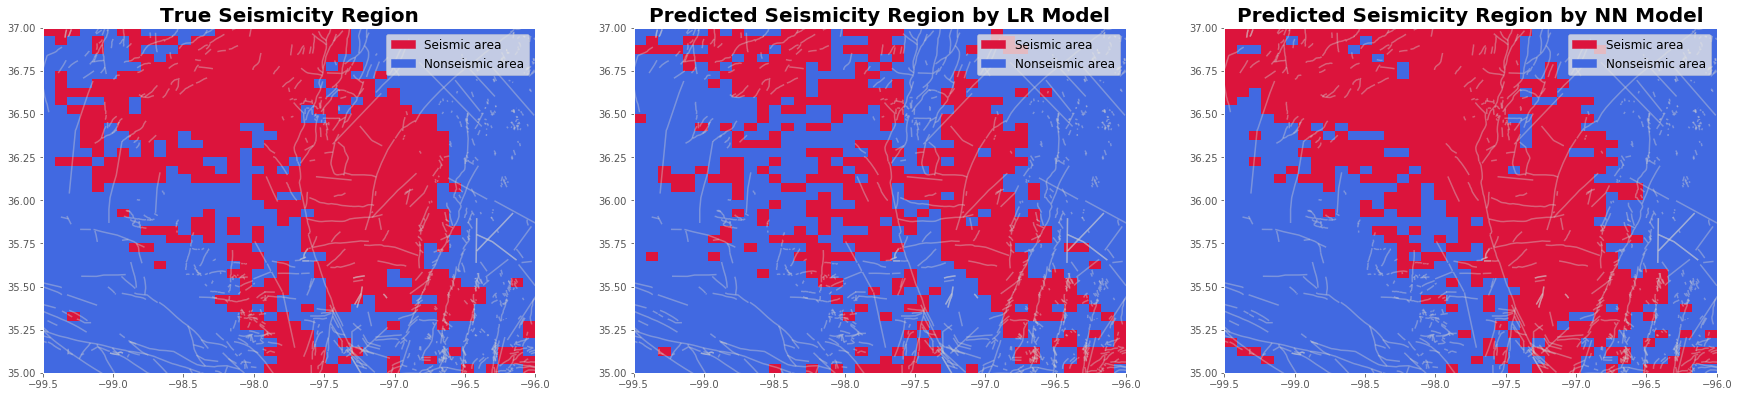
\includegraphics[width=1\textwidth]{mapping_comparison.png}
    \end{center}
    \caption{\label{fig:mapping_comparison} Seismicity prediction by logistic regression model and neural network model (The black line areas represent the interest areas where the performance compared between LR and NN model in Section~\ref{sec:model_evaluate_comparison}).}
\end{figure}

In the last part, we visualized the predictions by two models on Oklahoma map to make a more intuitive comparison.
The mapping results of predictions and mapping are shown in Figure~\ref{fig:mapping_comparison}. 
Both LR and NN model predicted the spatial distribution of major earthquake regional clusters mentioned in Section~\ref{sec:visualization_result}, even though the precision of regional outline is poor.
However, in terms of TPR, these two models performed greatly differently by predicted maps comparison with true map.
We want TPR (true positive rate) to be closer to 1 (equivalently FN closer to 0), which means we want to predict out more seismic regions among true seismic regions.
It is because we tend to regard an region at the risk of seismicity as seismic rather than nonseismic, in order to prevent the property damage and casualties.
According to Figure~\ref{fig:mapping_comparison}, all gridding regions in the two blocks marked by 1 and 2 are almost seismic (positive) in true seismic map.
NN model indeed selected out almost all true seismic regions in these two blocks, but LR model performs badly and wrongly predicts many seismic regions to be nonseismic.

\subsection{Feature Importance Analysis}
In this part, we will analyze the influence of each feature on earthquake prediction.
According to feature analysis by LR model and NN model in Figure~\ref{fig:feature_attribution}, we found the agreed main feature in them is \textit{the depth to basement}.
It shows that earthquake occurrence is negatively correlated with its depth to basement in that region.
Furthermore, \textit{well\_depth\_avg} (the average depth of active wells) and \textit{hf\_number} (the number of hydraulic fracturing activities) are also important features, which are positively correlated with seismicity in LR model but negatively correlated with seismicity in NN model.
This might be due to incomplete of dataset, or because LR model is so poorly fitted that the coefficient sign is wrong. Anyway, these two features should be further investigated in future work.
In NN model, in addition to three features above, we found that \textit{hf\_base\_water\_volume\_sum} is also considered to be important and negatively correlated with earthquake occurrence based on most attribution algorithms.
\begin{figure}
    \begin{center}
        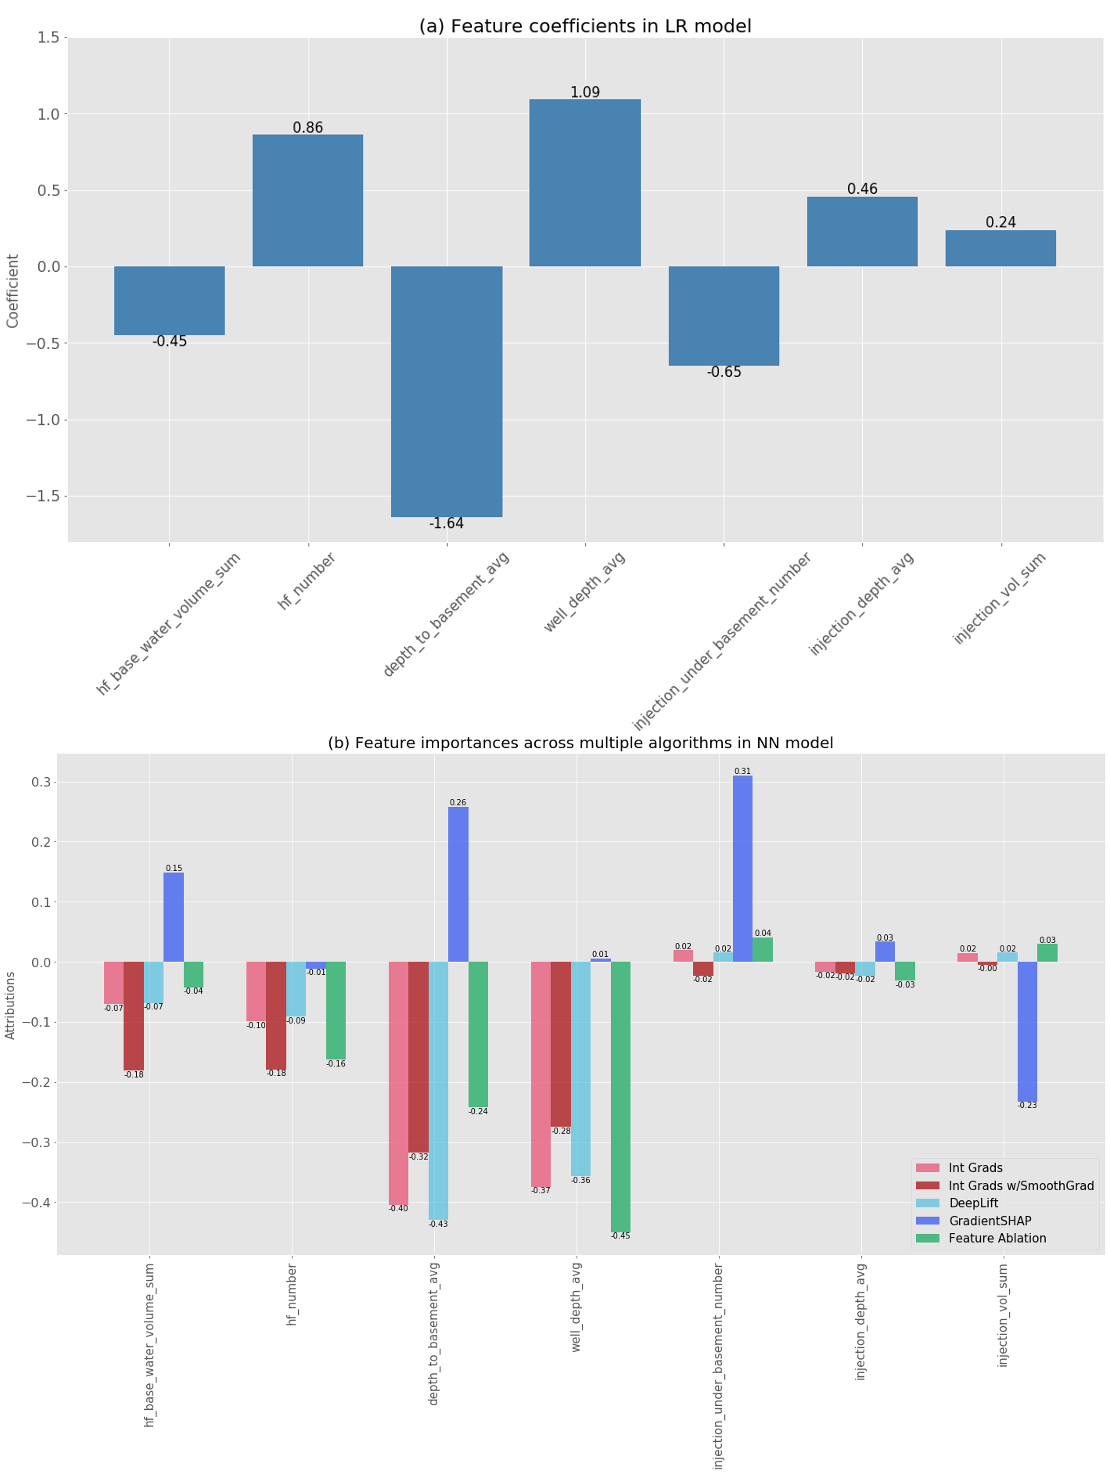
\includegraphics[width=1\textwidth]{feature_attribution.png}
    \end{center}
    \caption{\label{fig:feature_attribution} Feature attribution result by LR model and NN model.}
\end{figure}

\section{Conclusion and Future Work}
\label{sec:conclusion}
This project visualized various geological and industrial factors in Oklahoma and found some of them have rough correlations with seismicity. 
We selected out statistically significant features and eliminated multicollinearity by forward stepwise regression approach with VIF checking.
These features contain number of hydraulic fracturing activities, volume of water in hydraulic fracturing, depth to basement, depth of wells, volume of injections and number of injections deeper than basement.

Compared with physical model based on fluid flow and seismic physics by \citep{norbeck2018hydromechanical}, this project constructed two models using machine learning methods.
The logistic model works not badly in predicting non-seismic regions but have deficiencies in predicting seismic regions. 
The neural network model is good at predicting actual seismic areas in which we concentrate on.
According to the result map of interest area we selected, we concluded that neural network model trained can accurately predict out the most actual regions of the earthquake occurrence.
This is what logistic regression model cannot do. 

Through the feature importance analysis in LR model and NN model, we found the depth to basement is the key predictor of the spatial distribution of seismicity. 
It is consistent with both models that seismicity is largely promoted with the reduce in depth to basement.
The amount of hydraulic fracturing and the depth of wells are also found important but they have opposite correlation with seismicity among these two models, which require to be further investigated.
Furthermore, water volume in base of HF is additionally considered to be important and negatively correlated with earthquake occurrence through NN model.

We have implemented and tried to collect various data in a circular region with a radius of 10 km from the center in each rectangular gird point region.
For distance calculation in radius mode, we have tried two methods: One was using GeoPy module directly and the other was computing through distance formulas after cartesian coordinate mapping. 
However, they were time consuming (at least a few days cost) and not suitable for debugging my models. Due to the time limitation of this project, we only implemented the radius mode but actually used rectangular mode for training data generation. 
Therefore, we can use more reasonable radius mode for collecting features in future study, which may obtain ideal predictive performance and feature importance analysis. It might solve the partial inconsistencies of signs in the feature attribution section.

\newpage
% References
\bibliographystyle{agsm}
\bibliography{references.bib}  % BibTeX references are saved in references.bib

\newpage
% \appendix
\section*{Appendix}
\subsection{Supplementary Figures}

\begin{figure}[H]
    \begin{center}
        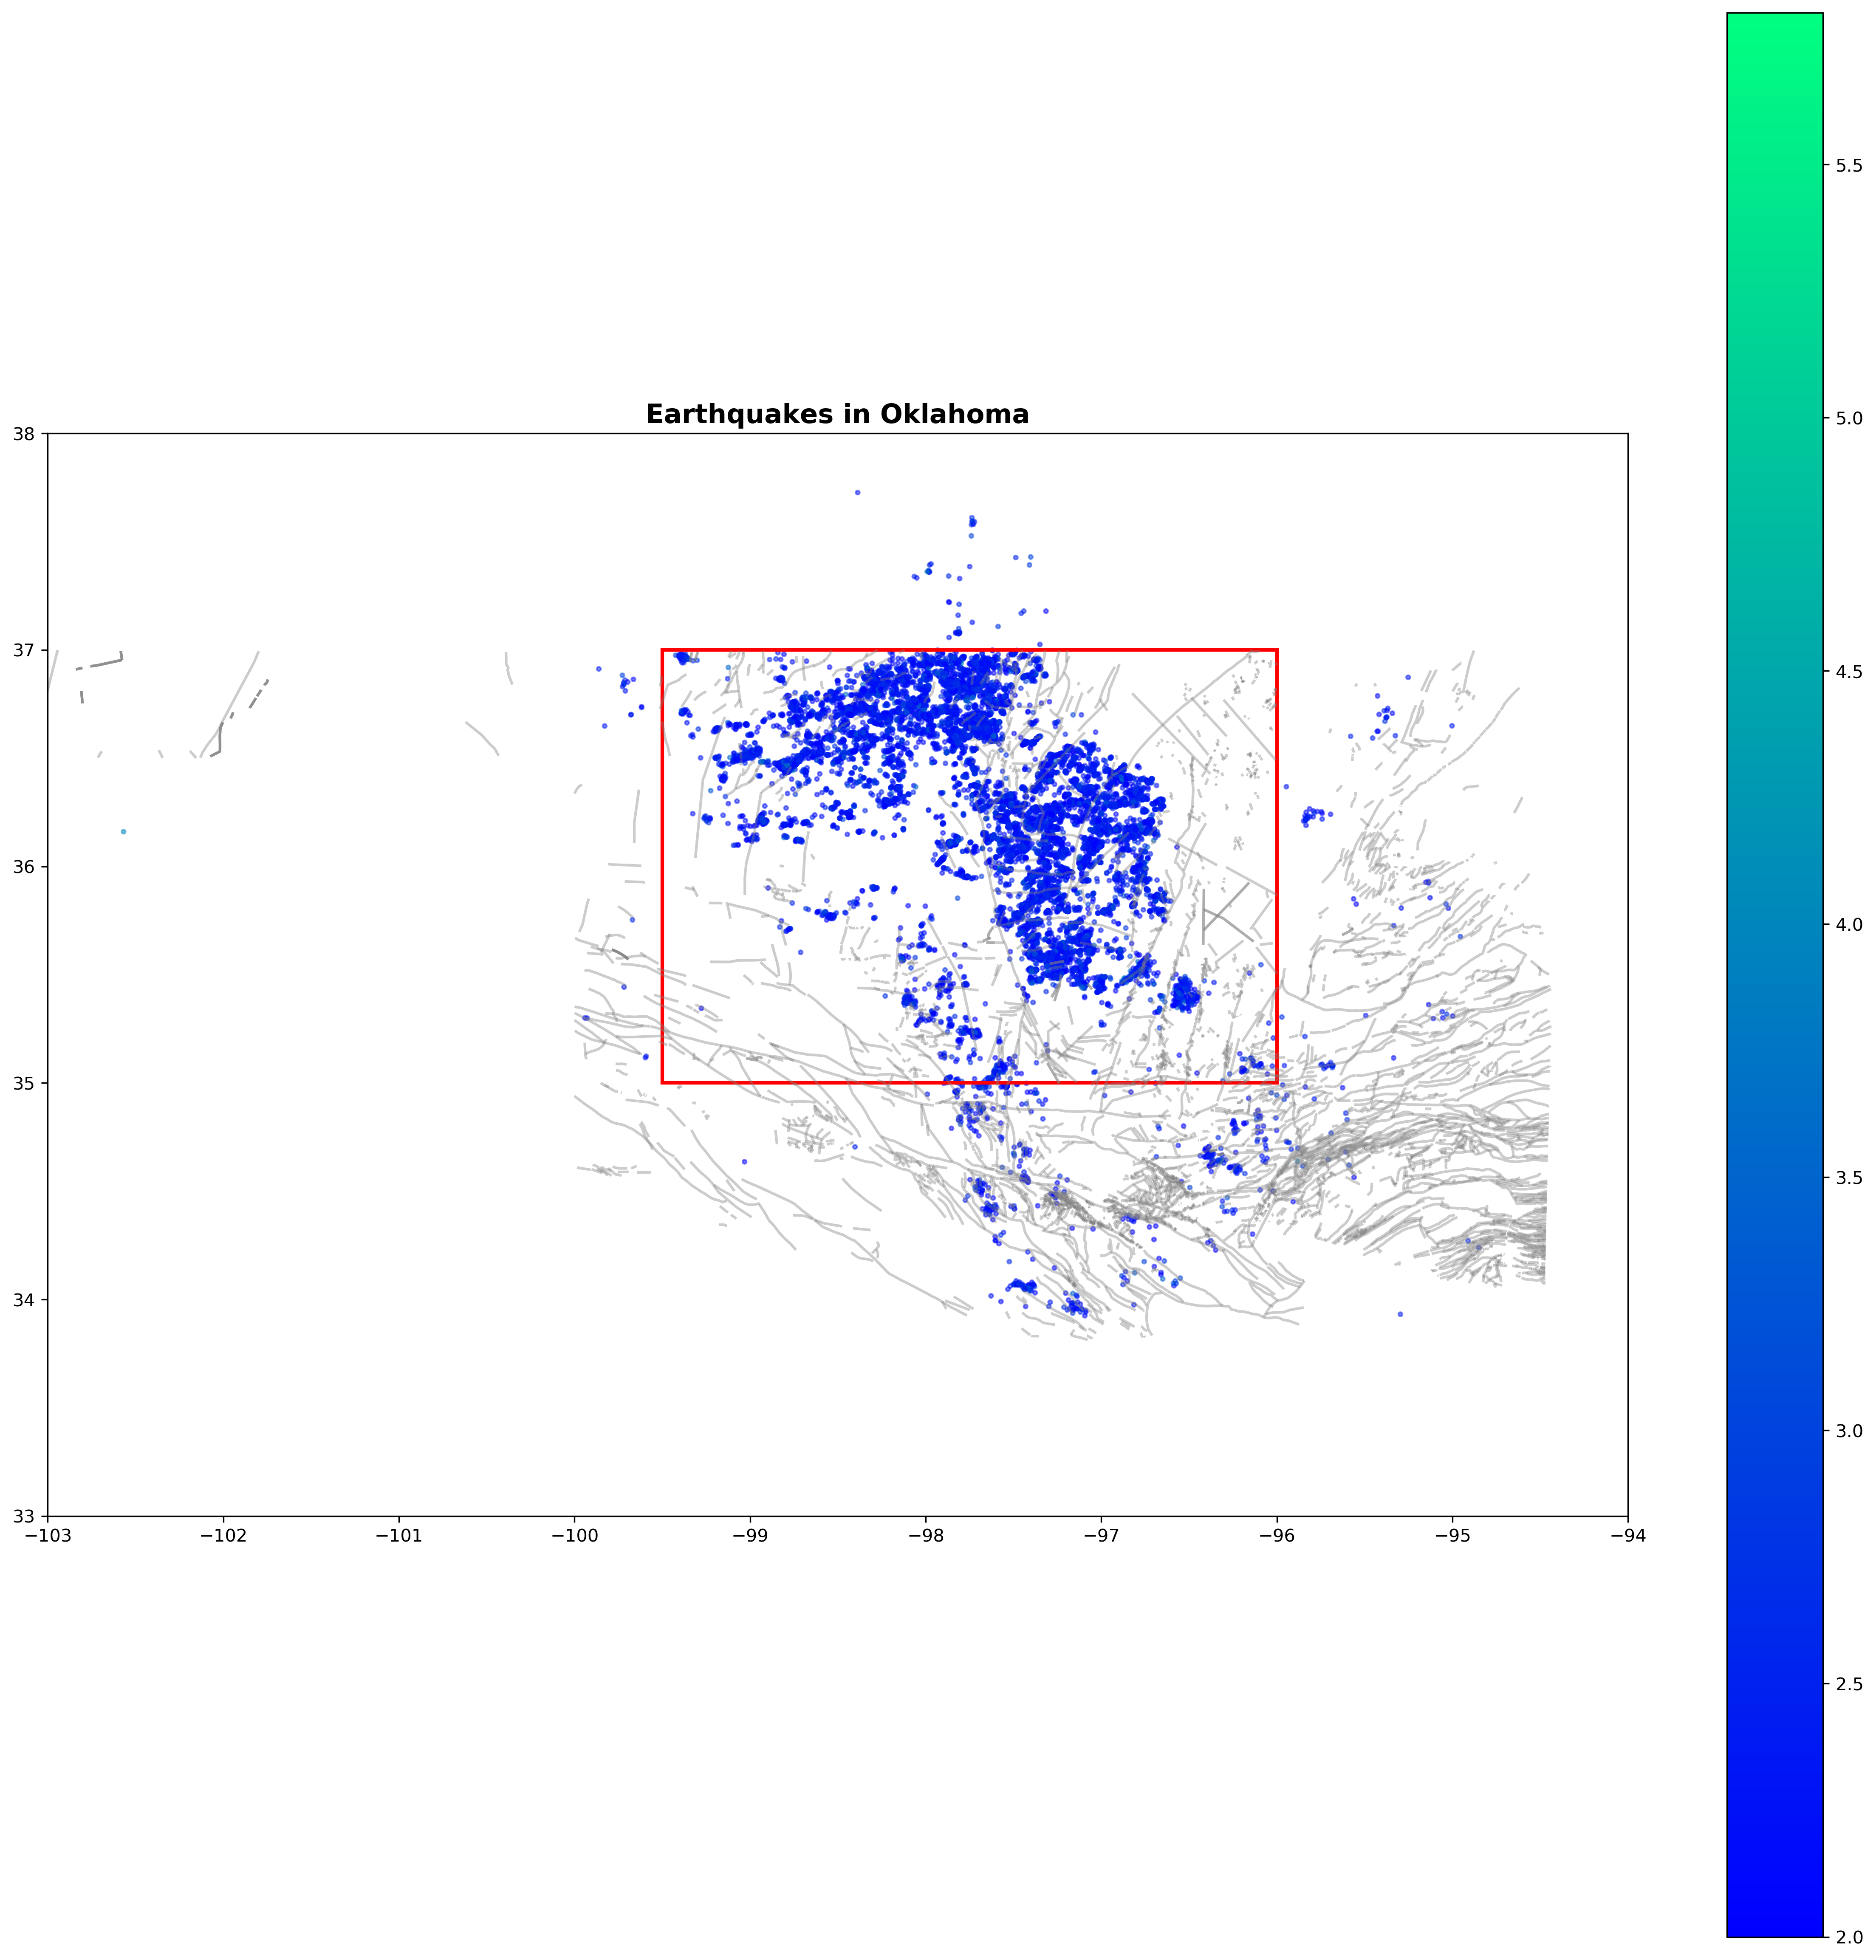
\includegraphics[width=0.8\textwidth]{earthquake_plot.png}
    \end{center}
    \caption{\label{fig:earthquake_plot} Earthquake occurrences in Oklahoma. The color of marker represents the magnitude of earthquake. The red box represents the interest area we studied in this project. The longitude ranges in (-99.5W, -96W) and latitude ranges in (35.0N, 37.0N)}
\end{figure}

% \begin{figure}[H]
%     \begin{center}
%         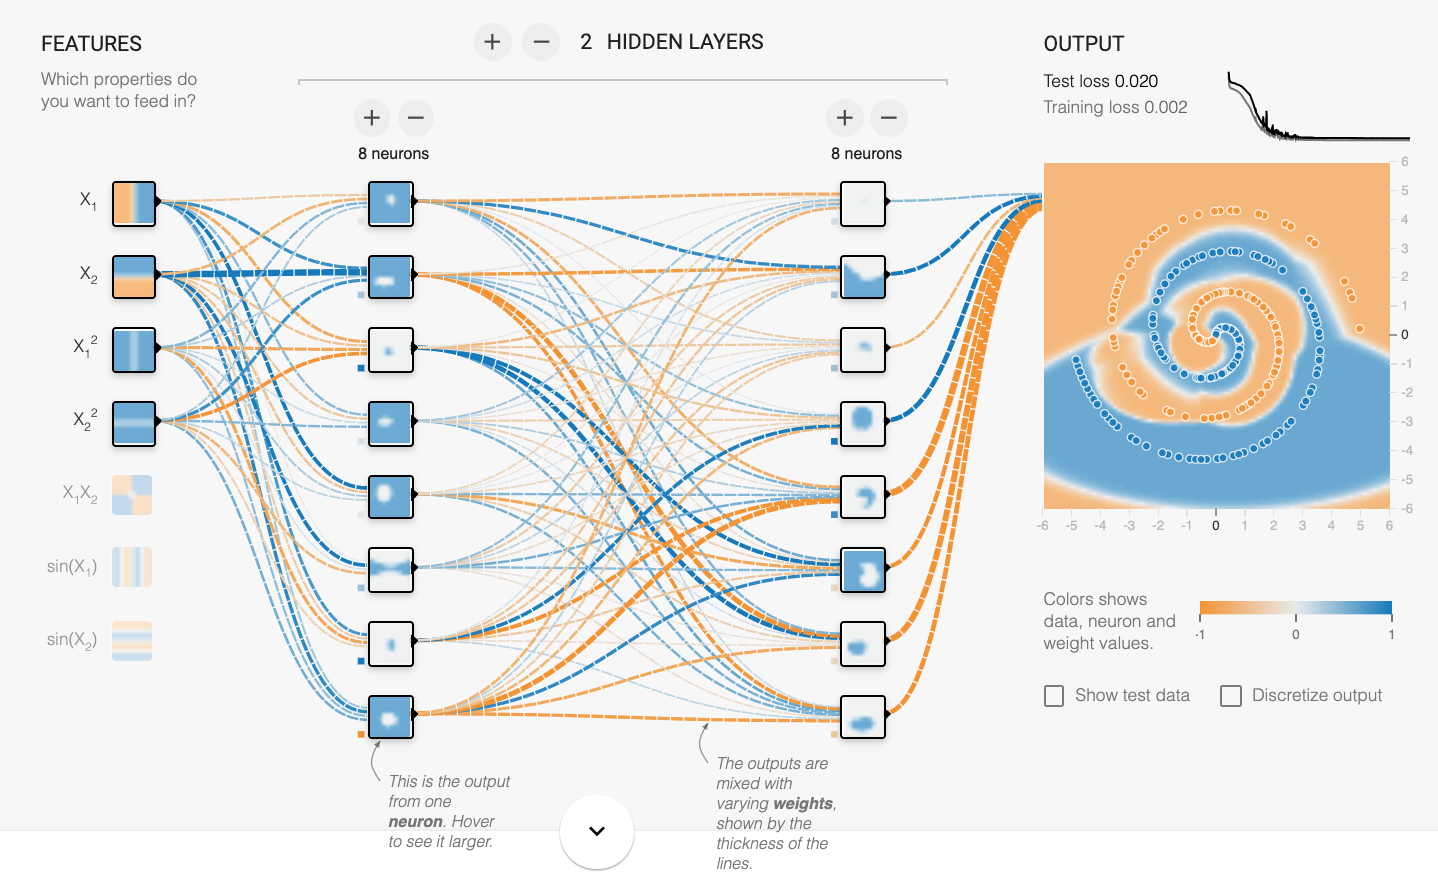
\includegraphics[width=1\textwidth]{neural_network_exmaple.png}
%     \end{center}
%     \caption{\label{fig:neural_network_example} The model created from above code simulated through playground.tensorflow.org}
% \end{figure}



\begin{figure}[H]
    \begin{center}
        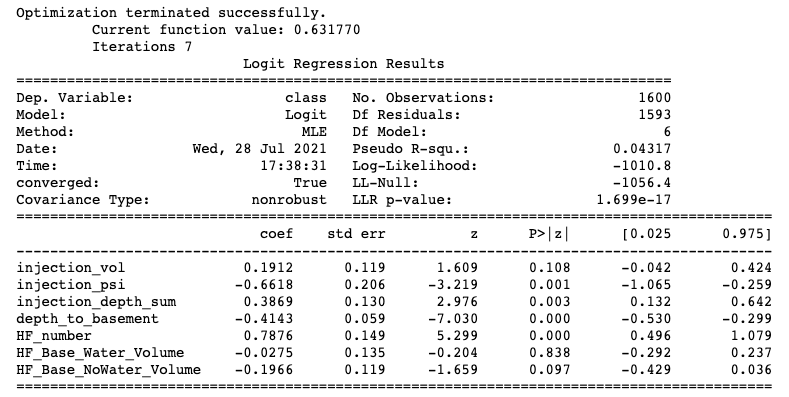
\includegraphics[width=1\textwidth]{p-value.png}
    \end{center}
    \caption{\label{fig:p-value} Feature selection in stepwise regression with p-value (It is an intermediate step in stepwise logistic regression process.
    The `injection\_vol', `HF\_Base\_Water\_Volume', `HF\_Base\_NoWater\_Volume' both have a p-value greater than threshold 0.05 in logistic regression results, which are not statistically significant and some of them should be eliminated properly in later process.)}
\end{figure}


% \begin{figure}[H]
%     \begin{center}
%         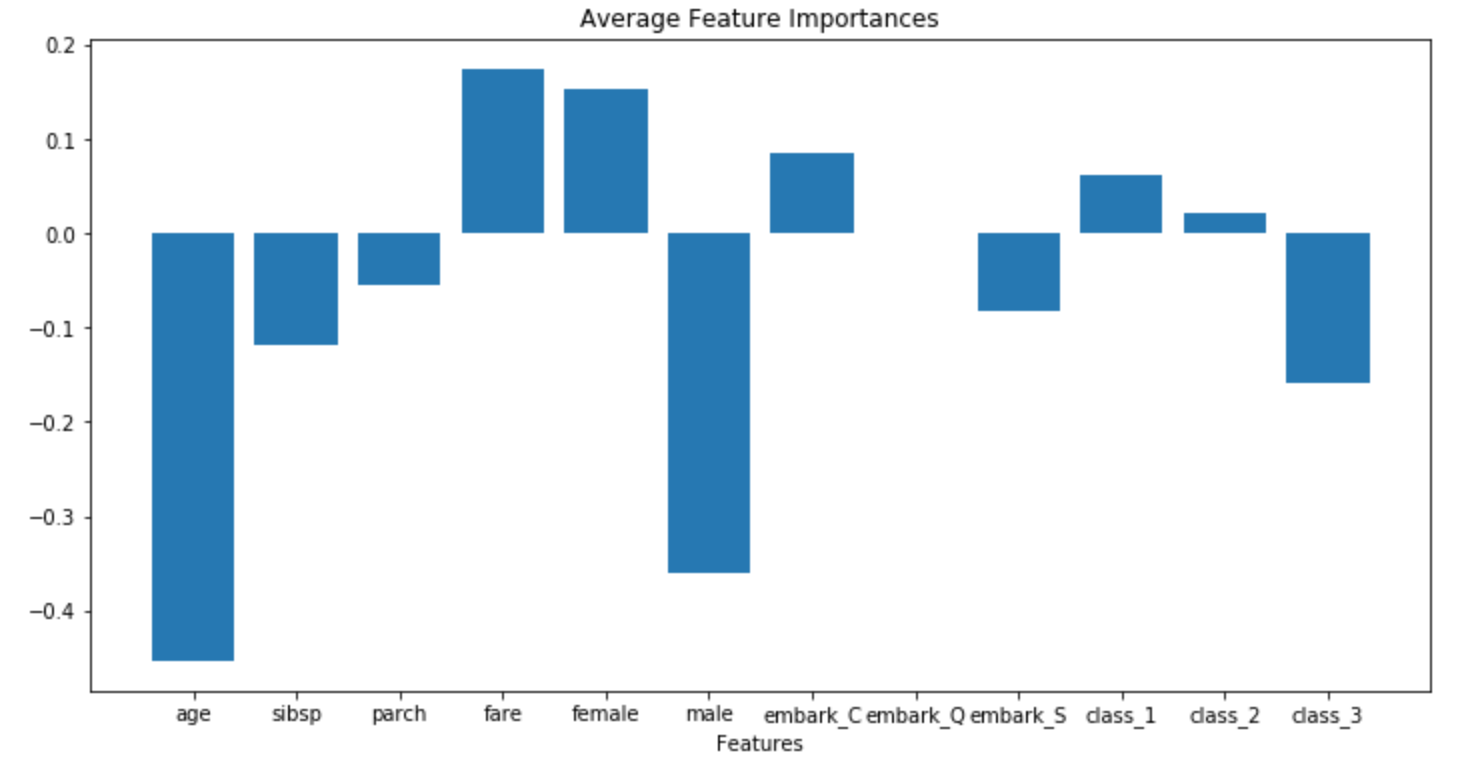
\includegraphics[width=1\textwidth]{feature_importance.png}
%     \end{center}
%     \caption{\label{fig:feature_importance} Feature importance example in Captum tutorial.}
% \end{figure}

\begin{figure}[H]
    \begin{center}
        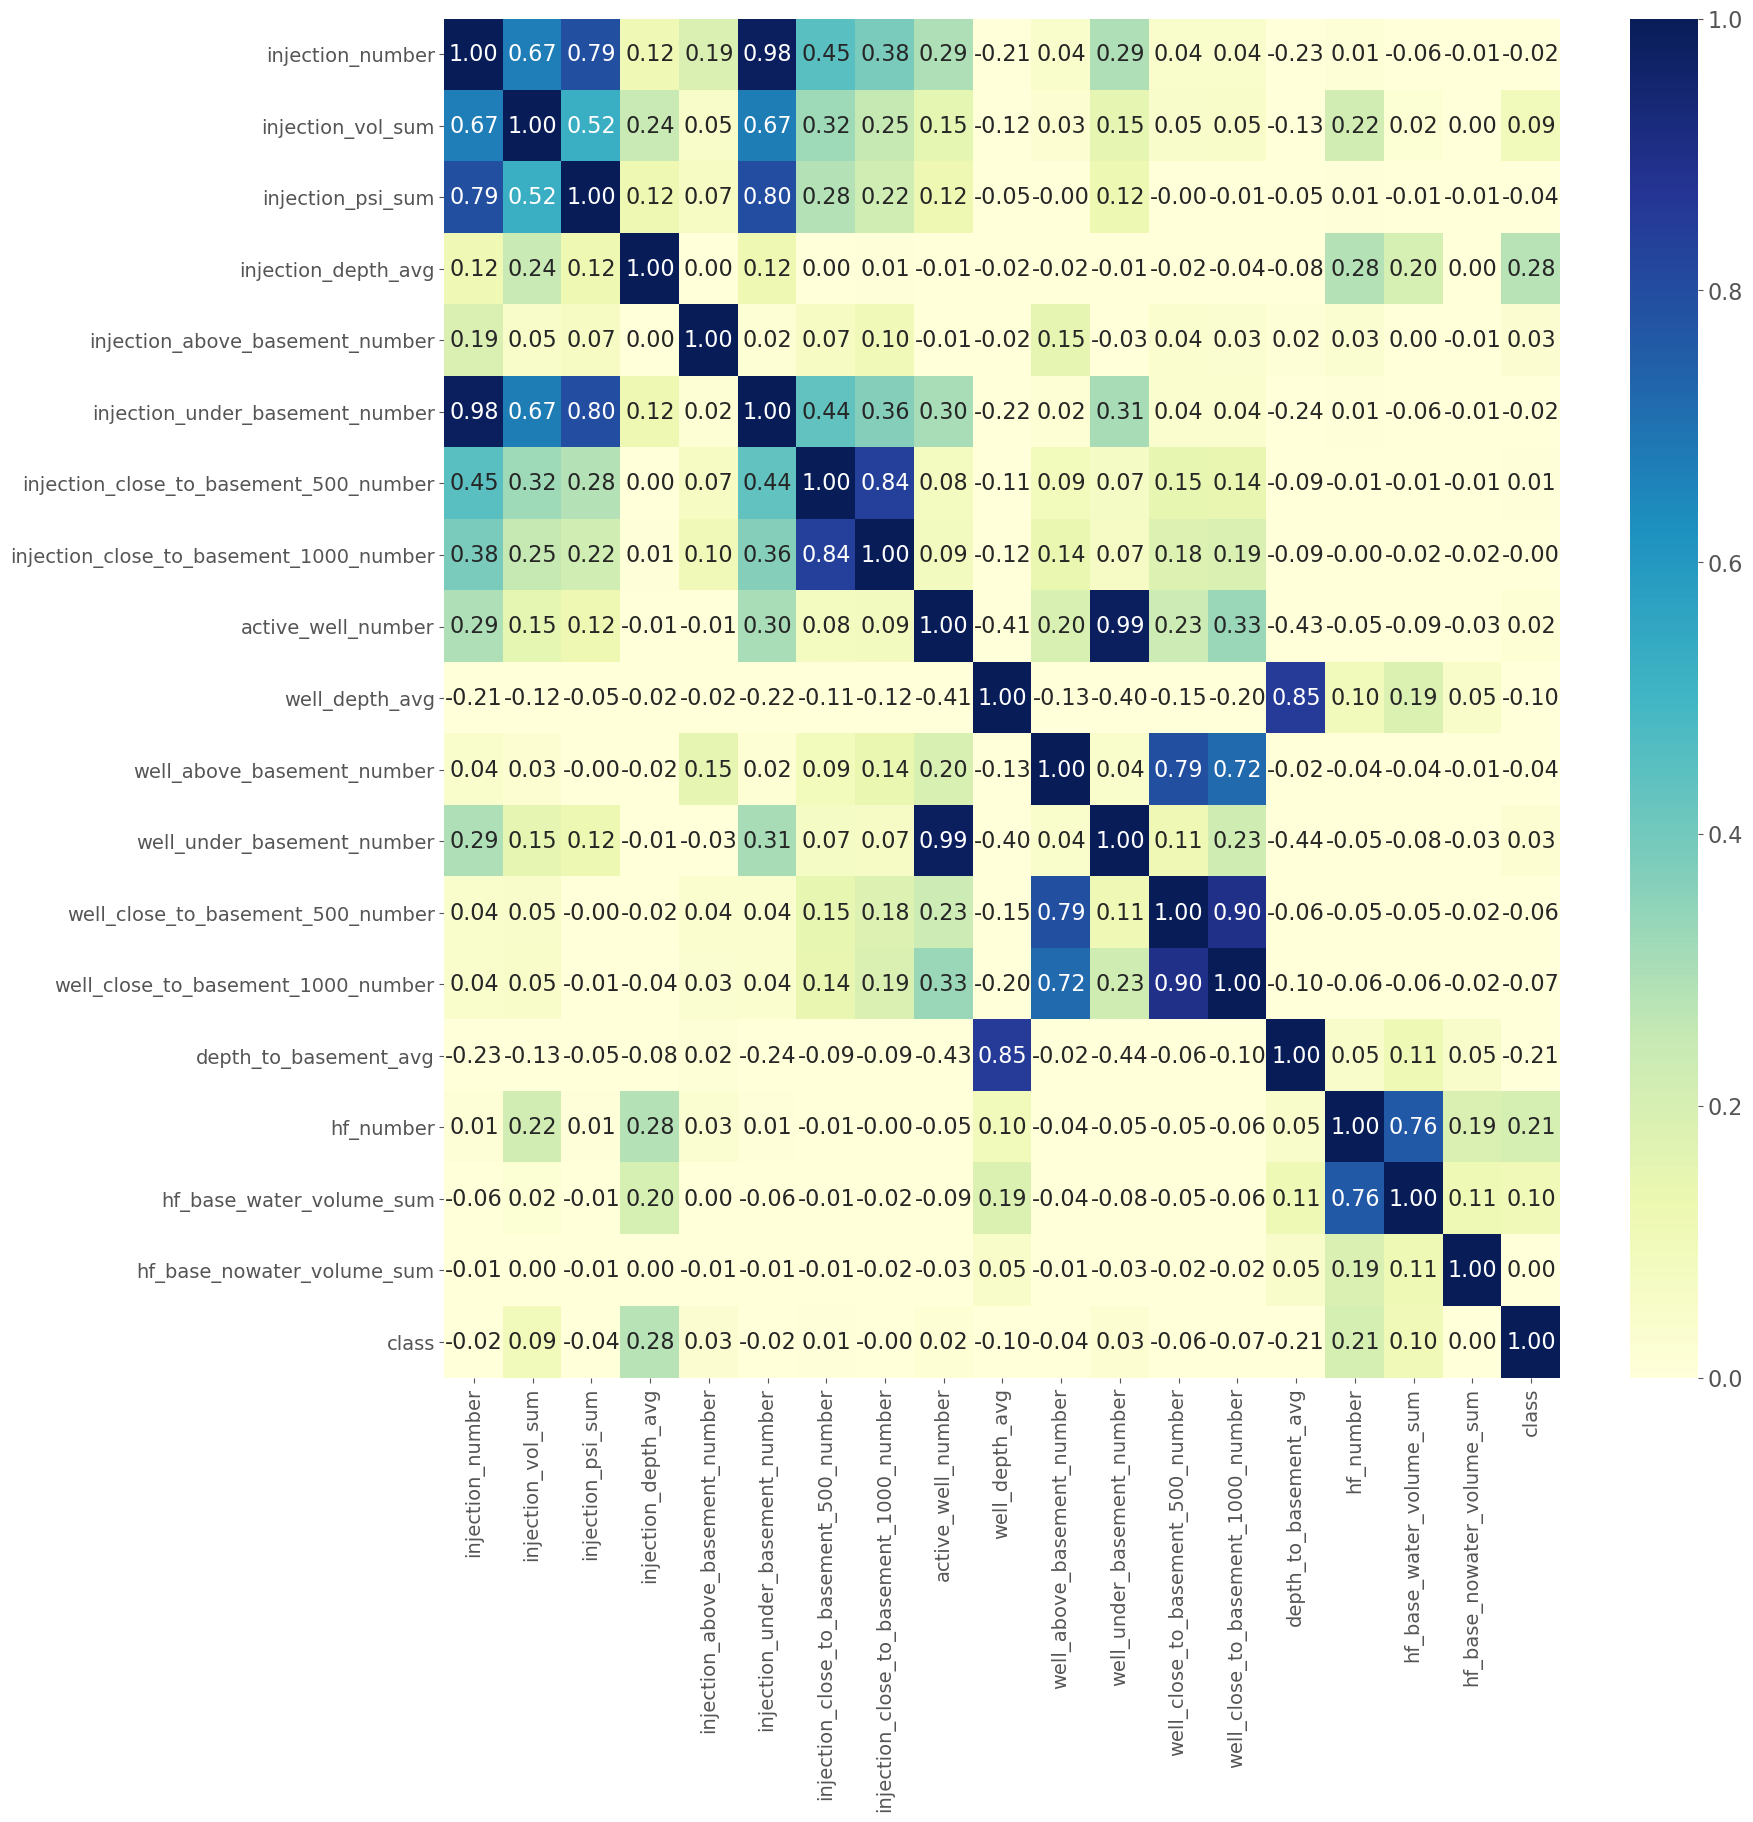
\includegraphics[width=1\textwidth]{heatmap_all.png}
    \end{center}
    \caption{\label{fig:heatmap} Correlation heatmap generated in Section~\ref{sec:SFSA}. We noted that there exists multicollinearity (dark blocks in figure) among these candidate features.}
\end{figure}

\begin{figure}[H]
    \begin{center}
        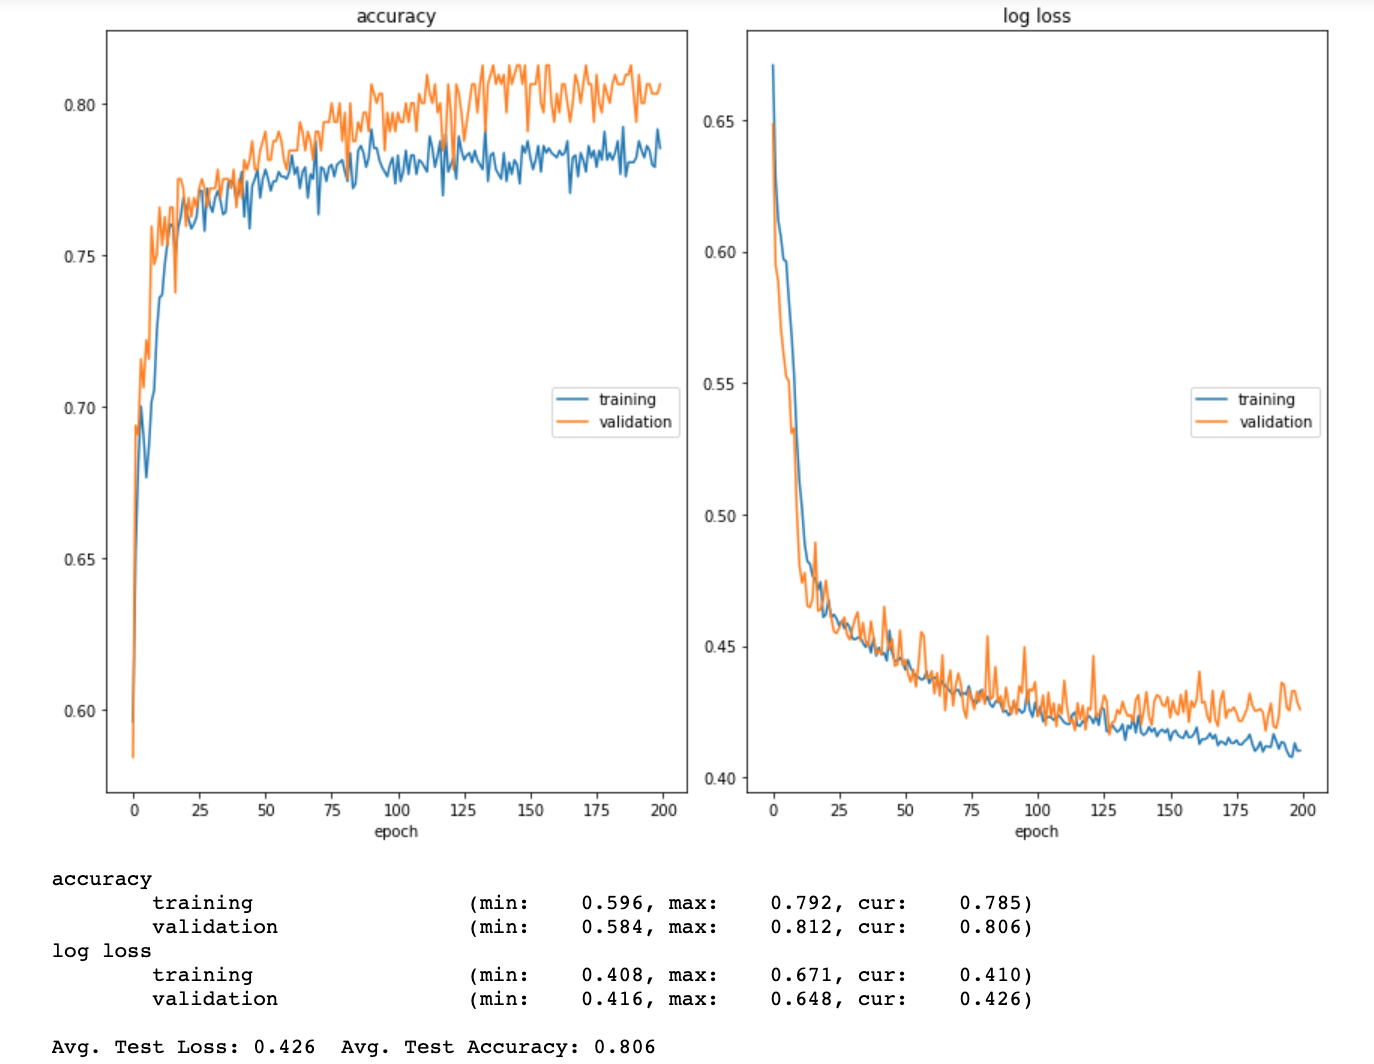
\includegraphics[width=1\textwidth]{training_process.png}
    \end{center}
    \caption{\label{fig:training_process} Neural network model training process in Section~\ref{sec:NN_training}. We stopped training when the log loss of the validation is no longer reduced. It means NN model is currently in an optimal trained state.}
\end{figure}

\subsection{Supplementary Tables}

\begin{table}[H]
    \centering
    \caption{The dependencies of this project}
    \label{tab:library_dependency}
    \begin{tabular}{|c|c|c|}
    \hline
    \textbf{Module} & \textbf{Version} & \textbf{Purpose}                                                                                                                                            \\ \hline
    os              & 3.7.11           & Search the data files (csv or xlsx) in the directory                                                                                                        \\ \hline
    numpy           & 1.18.1           & \multirow{2}{*}{Dataset process}                                                                                                                            \\ \cline{1-2}
    pandas          & 1.0.1            &                                                                                                                                                             \\ \hline
    Shapely         & 1.7.1            & \multirow{2}{*}{Map the activities on map in spatial}                                                                                                       \\ \cline{1-2}
    geopandas       & 0.9.0            &                                                                                                                                                             \\ \hline
    matplotlib      & 3.1.3            & \multirow{2}{*}{Plot the figure}                                                                                                                            \\ \cline{1-2}
    seaborn         & 0.10.0           &                                                                                                                                                             \\ \hline
    scipy           & 1.6.2            & \multirow{3}{*}{\begin{tabular}[c]{@{}c@{}}Load and process the geological formation data \\ and plot the figure\end{tabular}}                              \\ \cline{1-2}
    xarray          & 0.18.2           &                                                                                                                                                             \\ \cline{1-2}
    netCDF4         & 1.5.7            &                                                                                                                                                             \\ \hline
    statsmodels     & 0.12.2           & Used in stepwise regression                                                                                                                                 \\ \hline
    torch           & 1.9.0            & \multirow{3}{*}{\begin{tabular}[c]{@{}c@{}}Neural network model implementation and training, \\ and visualization of intermediate information\end{tabular}} \\ \cline{1-2}
    scikit-learn         & 0.22.1           &                                                                                                                                                             \\ \cline{1-2}
    livelossplot    & 0.5.4            &                                                                                                                                                             \\ \hline
    captum          & 0.4.0            & Perform the feature attribution                                                                                                                             \\ \hline
    \end{tabular}
    \end{table}

\begin{table}[]
    \centering
    \caption{Features generated by spatial gridding and data collecting for regions}
    \label{tab:feature_generated}
    \resizebox{\textwidth}{!}{%
    \begin{tabular}{|l|l|}
    \hline
    \multicolumn{1}{|c|}{Feature}                                     & \multicolumn{1}{c|}{Interpretation}                                    \\ \hline
    \textit{injection\_number {[}entry{]}}                            & the number of injections                                               \\ \hline
    \textit{injection\_vol\_sum {[}BPD{]}}                            & the sum of injection volume                                            \\ \hline
    \textit{injection\_psi\_sum {[}PSI{]}}                            & the sum of injection pressure                                          \\ \hline
    \textit{injection\_depth\_avg {[}m{]}}                            & the mean of injection depth                                            \\ \hline
    \textit{injection\_above\_basement\_number {[}entry{]}}           & the number of injections whose depth are shallow than the basement     \\ \hline
    \textit{injection\_under\_basement\_number {[}entry{]}}           & the number of injections whose depth are deeper than the basement      \\ \hline
    \textit{injection\_close\_to\_basement\_500\_number {[}entry{]}}  & the number of injections whose depth is within 500 metres of basement  \\ \hline
    \textit{injection\_close\_to\_basement\_1000\_number {[}entry{]}} & the number of injections whose depth is within 1000 metres of basement \\ \hline
    \textit{active\_well\_number {[}entry{]}}                         & the number of working wells                                            \\ \hline
    \textit{well\_depth\_avg {[}m{]}}                                 & the mean of well depth                                                 \\ \hline
    \textit{well\_above\_basement\_number {[}entry{]}}                & the number of working wells whose depth are shallow than the basement  \\ \hline
    \textit{well\_under\_basement\_number {[}entry{]}}                & the number of working wells whose depth are deeper than the basement   \\ \hline
    \textit{well\_close\_to\_basement\_500\_number {[}entry{]}}       & the number of wells whose depth is within 500 metres of basement       \\ \hline
    \textit{well\_close\_to\_basement\_1000\_number {[}entry{]}}      & the number of wells whose depth is within 1000 metres of basement      \\ \hline
    \textit{depth\_to\_basement\_avg {[}m{]}}                         & the mean of the depth to the basement                                  \\ \hline
    \textit{hf\_number {[}entry{]}}                                   & the number of hydraulic fracturing activities                          \\ \hline
    \textit{hf\_base\_water\_volume\_sum {[}BPD{]}}                   & the sum of volume by hydraulic fracturing with water                   \\ \hline
    \textit{hf\_base\_nowater\_volume\_sum {[}BPD{]}}                 & the sum of volume by hydraulic fracturing with nowater                 \\ \hline
    \textit{earthquake\_occurrence {[}0 or 1{]}}                       & 0: not occurred; 1: occurred.                                          \\ \hline
    \end{tabular}%
    }
    \end{table}

\subsection{Supplementary Codes and Results}
\subsubsection{The Code of Defining NN Model}
\label{sec:NN_code}
\begin{lstlisting}[language=Python]
    class Net(nn.Module):
    def __init__(self,n_input, n_output):
        super(Net,self).__init__()
        self.linear1 = nn.Linear(n_input, 8)
        self.relu1 = nn.ReLU()
        self.linear2 = nn.Linear(8, 8)
        self.relu2 = nn.ReLU()
        self.linear3 = nn.Linear(8, n_output)

    def forward(self, x):
        lin1_out = self.linear1(x)
        relu_out1 = self.relu1(lin1_out)
        relu_out2 = self.relu2(self.linear2(relu_out1))
        return self.linear3(relu_out2)
\end{lstlisting}

\subsubsection{The Process in Stepwise Regression with VIF Checking}
\label{sec:feature_selection_process}
\begin{itemize}
    \item \textit{Iteration 1}\\
    Feature selected: hf\_base\_nowater\_volume\_sum\\
    P-value \textgreater 0.05 check: hf\_base\_nowater\_volume\_sum\\
    Feature removed: hf\_base\_nowater\_volume\_sum\\
    VIF\textgreater 5 check: None\\
    Feature removed: None
    
    \item \textit{Iteration 2}\\
    Feature selected: hf\_base\_water\_volume\_sum\\
    P-value \textgreater 0.05 check: None\\
    Feature removed: None\\
    VIF\textgreater 5 check: None\\
    Feature removed: None\\
    
    \item \textit{Iteration 3}\\
    Feature selected: hf\_number\\
    P-value \textgreater 0.05 check: None\\
    Feature removed: None\\
    VIF\textgreater 5 check: None\\
    Feature removed: None\\
    
    \item \textit{Iteration 4}\\
    Feature selected: depth\_to\_basement\_avg\\
    P-value \textgreater 0.05 check: None\\
    Feature removed: None\\
    VIF\textgreater 5 check: None\\
    Feature removed: None\\
    
    \item \textit{Iteration 5}\\
    Feature selected: well\_close\_to\_basement\_1000\_number\\
    P-value \textgreater 0.05 check: None\\
    Feature removed: None\\
    VIF\textgreater 5 check: None\\
    Feature removed: None\\
    
    \item \textit{Iteration 6}\\
    Feature selected: well\_close\_to\_basement\_500\_number\\
    P-value \textgreater 0.05 check: well\_close\_to\_basement\_500\_number(0.647), well\_close\_to\_basement\_1000\_number(0.065)\\
    Feature removed: well\_close\_to\_basement\_500\_number\\
    VIF\textgreater 5 check: None\\
    Feature removed: None\\
    
    
    \item \textit{Iteration 7}\\
    Feature selected: well\_under\_basement\_number\\
    P-value \textgreater 0.05 check: None\\
    Feature removed: None\\
    VIF\textgreater 5 check: None\\
    Feature removed: None\\
    
    \item \textit{Iteration 8}\\
    Feature selected: well\_above\_basement\_number\\
    P-value \textgreater 0.05 check: well\_above\_basement\_number(0.46)\\
    Feature removed: well\_above\_basement\_number\\
    VIF\textgreater 5 check: None\\
    Feature removed: None\\
    
    \item \textit{Iteration 9}\\
    Feature selected: well\_depth\_avg\\
    P-value \textgreater 0.05 check: well\_close\_to\_basement\_1000\_number(0.352)\\
    Feature removed: well\_close\_to\_basement\_1000\_number\\
    VIF\textgreater 5 check: None\\
    Feature removed: None\\
    
    \item \textit{Iteration 10}\\
    Feature selected: active\_well\_number\\
    P-value \textgreater 0.05 check:  well\_under\_basement\_number(0.477), active\_well\_number(0.772)\\
    Feature removed: active\_well\_number\\
    VIF\textgreater 5 check: None\\
    Feature removed: None\\
    
    \item \textit{Iteration 11}\\
    Feature selected: injection\_close\_to\_basement\_1000\_number\\
    P-value \textgreater 0.05 check: injection\_close\_to\_basement\_1000\_number(0.876)\\
    Feature removed: injection\_close\_to\_basement\_1000\_number\\
    VIF\textgreater 5 check: None\\
    Feature removed: None\\
    
    
    \item \textit{Iteration 12}\\
    Feature selected: injection\_close\_to\_basement\_500\_number\\
    P-value \textgreater 0.05 check: injection\_close\_to\_basement\_500\_number(0.876)\\
    Feature removed: injection\_close\_to\_basement\_500\_number\\
    VIF\textgreater 5 check: None\\
    Feature removed: None\\
    
    \item \textit{Iteration 13}\\
    Feature selected: injection\_under\_basement\_number\\
    P-value \textgreater 0.05 check: well\_under\_basement\_number(0.102)\\
    Feature removed: well\_under\_basement\_number\\
    VIF\textgreater 5 check: None\\
    Feature removed: None\\
    
    
    \item \textit{Iteration 14}\\
    Feature selected: injection\_above\_basement\_number\\
    P-value \textgreater 0.05 check: None\\
    Feature removed: None\\
    VIF\textgreater 5 check: None\\
    Feature removed: None\\
    
    \item \textit{Iteration 15}\\
    Feature selected: injection\_depth\_avg\\
    P-value \textgreater 0.05 check: injection\_above\_basement\_number\\
    Feature removed: injection\_above\_basement\_number\\
    VIF\textgreater 5 check: None\\
    Feature removed: None\\
    
    \item \textit{Iteration 16}\\
    Feature selected: injection\_psi\_sum\\
    P-value \textgreater 0.05 check: injection\_psi\_sum(0.969)\\
    Feature removed: injection\_psi\_sum\\
    VIF\textgreater 5 check: None\\
    Feature removed: None\\
    
    \item \textit{Iteration 17}\\
    Feature selected: injection\_vol\_sum\\
    P-value \textgreater 0.05 check: None\\
    Feature removed: None\\
    VIF\textgreater 5 check: None\\
    Feature removed: None\\
    
    \item \textit{Iteration 18}\\
    Feature selected: injection\_number\\
    P-value \textgreater 0.05 check: injection\_under\_basement\_number(0.065), injection\_number(0.194)\\
    Feature removed: injection\_number\\
    VIF\textgreater 5 check: None\\
    Feature removed: None\\
    \end{itemize}

\end{document}


